\documentclass[xcolor=dvipsnames, aspectratio=1610]{beamer}
%{{{
\usepackage{amsmath,amssymb,graphicx,float,dsfont,fancybox}
\usepackage{BeamerColor}

%\usetheme{Warsaw}
%\usetheme[secheader]{Boadilla}
\usetheme{default}
\usecolortheme[named=DarkSeaGreen4]{structure}
    \setbeamertemplate{footline}[frame number]

\beamertemplatenavigationsymbolsempty
\useinnertheme{rectangles} % Vierecke
\setbeamertemplate{itemize items}[circle]
\setbeamertemplate{sections/subsections in toc}[circle]
\usesubitemizeitemtemplate{%
    \tiny\raise1.5pt\hbox{\color{beamerstructure}${\boldsymbol \diamond}$}%
}

\usefonttheme{default}
\usepackage{relsize}
\setbeamertemplate{blocks}[default]
\usepackage{slashed}
\usepackage{ulem}

\usepackage{amsmath}
\usepackage{amsfonts}
\usepackage{amssymb}
\usepackage{amsmath,bm}
\usepackage{wasysym}
\usepackage{color}
\usepackage{movie15}
\usepackage{appendixnumberbeamer}
\usepackage{listings}
\usepackage{exscale,relsize}
\usepackage{cancel}
\usepackage{setspace}
\usepackage{tikz}
\usetikzlibrary{decorations.pathreplacing}
\usetikzlibrary{calc,shapes.callouts,shapes.arrows}
\usetikzlibrary{shapes,snakes}
\usetikzlibrary{positioning}
\usetikzlibrary{arrows}
\usetikzlibrary{backgrounds}


\usepackage{animate}
\usepackage{graphics} 


\newcommand{\tikzmark}[1]{\tikz[overlay,remember picture] \node (#1) {};}
\newcommand{\arrowthis}[2]{
        \tikz[remember picture,baseline]{\node[anchor=base,inner sep=0,outer sep=0]%
        (#1) {\underline{#1}};
        \node[overlay,single arrow,draw=none,fill=red!50,anchor=tip,rotate=60]
        at (#1.south) {#2};}%
    }%
\newcommand{\speechthis}[2]{
        \tikz[remember picture,baseline]{\node[anchor=base,inner sep=0,outer sep=0]%
        (#1) {\underline{#1}};\node[overlay,ellipse callout,fill=blue!50]
        at ($(#1.north)+(-.5cm,0.8cm)$) {#2};}%
    }%
\newcommand{\cloudethis}[2]{
        \tikz[remember picture,baseline]{\node[anchor=base,inner sep=0,outer sep=0]%
        (#1) {\underline{#1}};\node[overlay,cloud callout,callout relative pointer={(0.2cm,-0.7cm)},%
        aspect=2.5,fill=yellow!90] at ($(#1.north)+(-0.5cm,1.6cm)$) {#2};}%
    }%
\newcommand{\pointthis}[2]{
        \tikz[remember picture,baseline]{
        \node[anchor=base,inner sep=0,outer sep=0](#1) {#1};
        \node[overlay,ellipse,fill=Cerulean!50] at ($(#1.north)+(0.2cm,-0.5cm)$) {\color{black}\tiny{#2}};}%
        }%
\newcommand{\talkabove}[3]{
        \tikz[remember picture,baseline]{
        \node[anchor=base,inner sep=0,outer sep=0](#1) {{\color{#3}#1}};
        \node[overlay,ellipse,fill=#3!50] at ($(#1.north)+(0.2cm,+0.4cm)$) {\color{black}\tiny{#2}};}%
        }%
\newcommand{\talkbelow}[2]{
        \tikz[remember picture,baseline]{
        \node[anchor=base,inner sep=0,outer sep=0](#1) {#1};
        \node[overlay,ellipse,fill=Cerulean!50] at ($(#1.north)+(0.2cm,-0.5cm)$) {\color{black}\tiny #2};}%
        }%
\newcommand{\mylabel}[3]{
        \tikz[remember picture,baseline]{
        \node[ellipse] at (#1cm,#2cm) {\color{black}\tiny #3};}%
        }%
\newcommand{\bubblethis}[2]{
        \tikz[remember picture,baseline]{\node[anchor=base,inner sep=0,outer sep=0]%
        (#1) {\underline{#1}};\node[overlay,ellipse,fill=green!50] at ($(#1.north)+(-.5cm,-1.4cm)$) {#2};}%
        }%
\definecolor{alertAcolor}{rgb}{0.9 .1 0.7}
\newcommand{\alertA}[1]{\color{alertAcolor}#1\color{Black}}
%%----------------------------------------------
%%   My Colors
\definecolor{CL68}{rgb}{0,0.5,0}
\definecolor{CL95}{rgb}{0.6,1,0.6}

\definecolor{HPScol}{RGB}{255, 170, 220} 
\definecolor{DarkLightcol}{rgb}{0,0,1} 
\definecolor{Alertcol}{rgb}{1,0.1,0.3}
\definecolor{AlertcolB}{rgb}{0.4,0.2,0.9}
\definecolor{Eqcol}{rgb}{0,0.6,0.3}
\definecolor{Refcol}{rgb}{0.8,0.5,0.25}
\definecolor{quitegray}{rgb}{0.5,0.5,0.5}
\definecolor{springgreen}{rgb}{0.4,0.7,0.55}
\definecolor{OmegaDMcol}{RGB}{150,255,150} 
\definecolor{grcol}{rgb}{0.5,0.5,0.5}

\def \SerpC {RoyalBlue}
\def \AC {Salmon}
\def \gC {RedOrange}
\def \SMPMC {Green}
\def \EC {Fuchsia}
\def \APEXC {Purple}
\def \HPSC {HPScol}
\def \MESAC {Cyan}
\def \DLC {DarkLightcol}
\def \OrsayC {DarkLightcol}
%%----------------------------------------------
%%   My Commands
\renewcommand{\alert}[1]{{\color{Alertcol}#1}}
\newcommand{\alertC}[1]{{\color{RoyalBlue}#1}}

\newcommand{\HS}{{\color{HScol}HS }}
\newcommand{\headcol}[1]{{\color{JungleGreen}#1}}
\newcommand{\alertB}[1]{{\color{AlertcolB}#1}}
\newcommand{\eqc}[1]{{\color{Eqcol}#1}}
\newcommand{\gr}[1]{{\color{grcol}#1}}

\newcommand{\refc}[1]{{\color{Tan}#1}}
\newcommand{\myref}[1]{{\refc{\textsuperscript{\tiny{#1}} } }}
\newcommand{\myitem}{{\color{JungleGreen}\tiny{$\blacksquare$} }}
\newcommand{\putTxt}[2]{{\color{#1}\textrm{\tiny{#2}} }}
\newcommand{\putCaps}[2]{{\color{#1}\textsc{\tiny{#2}} }}
\newcommand{\bra}[1]{\left\langle{#1}\right\vert}
\newcommand{\ket}[1]{\left\vert{#1}\right\rangle}
\newcommand{\LA}{
\includegraphics[width=0.85cm]{Figures/ArrowL.jpg}\;\;}
\newcommand{\RA}{\raisebox{-0.1cm}{
\includegraphics[width=0.85cm]{Figures/ArrowS.jpg}\;\;}}
\newcommand{\RD}{
\includegraphics[width=0.85cm]{Figures/ArrowD.jpg}\;\;}
\newcommand{\RU}{
\includegraphics[width=0.85cm]{Figures/ArrowU.jpg}\;\;}
\newcommand{\RB}{
\includegraphics[width=0.45cm]{Figures/ArrowN.jpg}\;\;}

\newcommand\mysymb{\scalebox{.4}{(}\raisebox{-1.6pt}{$-$}\scalebox{.4}{)}}

\newcommand{\citeWork}[1]{ {\scriptsize{\color{Refcol} #1  \color{Black}}}}

    \newcommand\brabar{\raisebox{-4.0pt}{\scalebox{.2}{
    			\textbf{(}}}\raisebox{-4.0pt}{{\_}}\raisebox{-4.0pt}{\scalebox{.2}{\textbf{\;)
    			}}}}

\def \azeL{ \alert{{A_0^L}}    }
\def \azeR{ \alert{{A_0^R}}    }
\def \apaL{ \alert{{A_\|^L}}   }
\def \apaR{ \alert{{A_\|^R}}   }
\def \apeL{ \alert{{A_\bot^L}} }
\def \apeR{ \alert{{A_\bot^R}} }


%%----------------------------------------------
%%   Get Started
\makeatletter
\newenvironment{customlist}[2]{
  \ifnum\@itemdepth >2\relax\@toodeep\else
      \advance\@itemdepth\@ne%
      \beamer@computepref\@itemdepth%
      \usebeamerfont{itemize/enumerate \beameritemnestingprefix body}%
      \usebeamercolor[fg]{itemize/enumerate \beameritemnestingprefix body}%
      \usebeamertemplate{itemize/enumerate \beameritemnestingprefix body begin}%
      \begin{list}
        {
            \usebeamertemplate{itemize \beameritemnestingprefix item}
        }
        { \leftmargin=#1 \labelsep=#2
            \def\makelabel##1{%
              {%
                  \hss\llap{{%
                    \usebeamerfont*{itemize \beameritemnestingprefix item}%
                        \usebeamercolor[fg]{itemize \beameritemnestingprefix item}##1}}%
              }%
            }%
        }
  \fi
}
{
  \end{list}
  \usebeamertemplate{itemize/enumerate \beameritemnestingprefix body end}%
}
\makeatother


%------------------------------------------------------------------------------------------------------------
%------------------------------------------------------------------------------------------------------------
%   Begin Document
%------------------------------------------------------------------------------------------------------------
%------------------------------------------------------------------------------------------------------------
\begin{document}


\title[Bob Andrews]{Example pattern extraction from text with a convolutional neural network}
\author{ch
}
\institute{}
\date[Hamburg, 2018]{{\small{2018}} \\ {\tiny{$~$}} \vspace{-0.2cm} \\{\bf internal}}
\begin{frame}
\begin{minipage}{0.49\textwidth}
\vspace{-0.2mm}

\end{minipage}
\begin{minipage}{0.49\textwidth}
\titlepage
\citeWork{https://github.com/chambrock/bob-andrews}
\begin{center}
\end{center}
\end{minipage}
\end{frame}






\begin{frame}{input data}
\linespread{1}\large{
\begin{minipage}{1\textwidth}
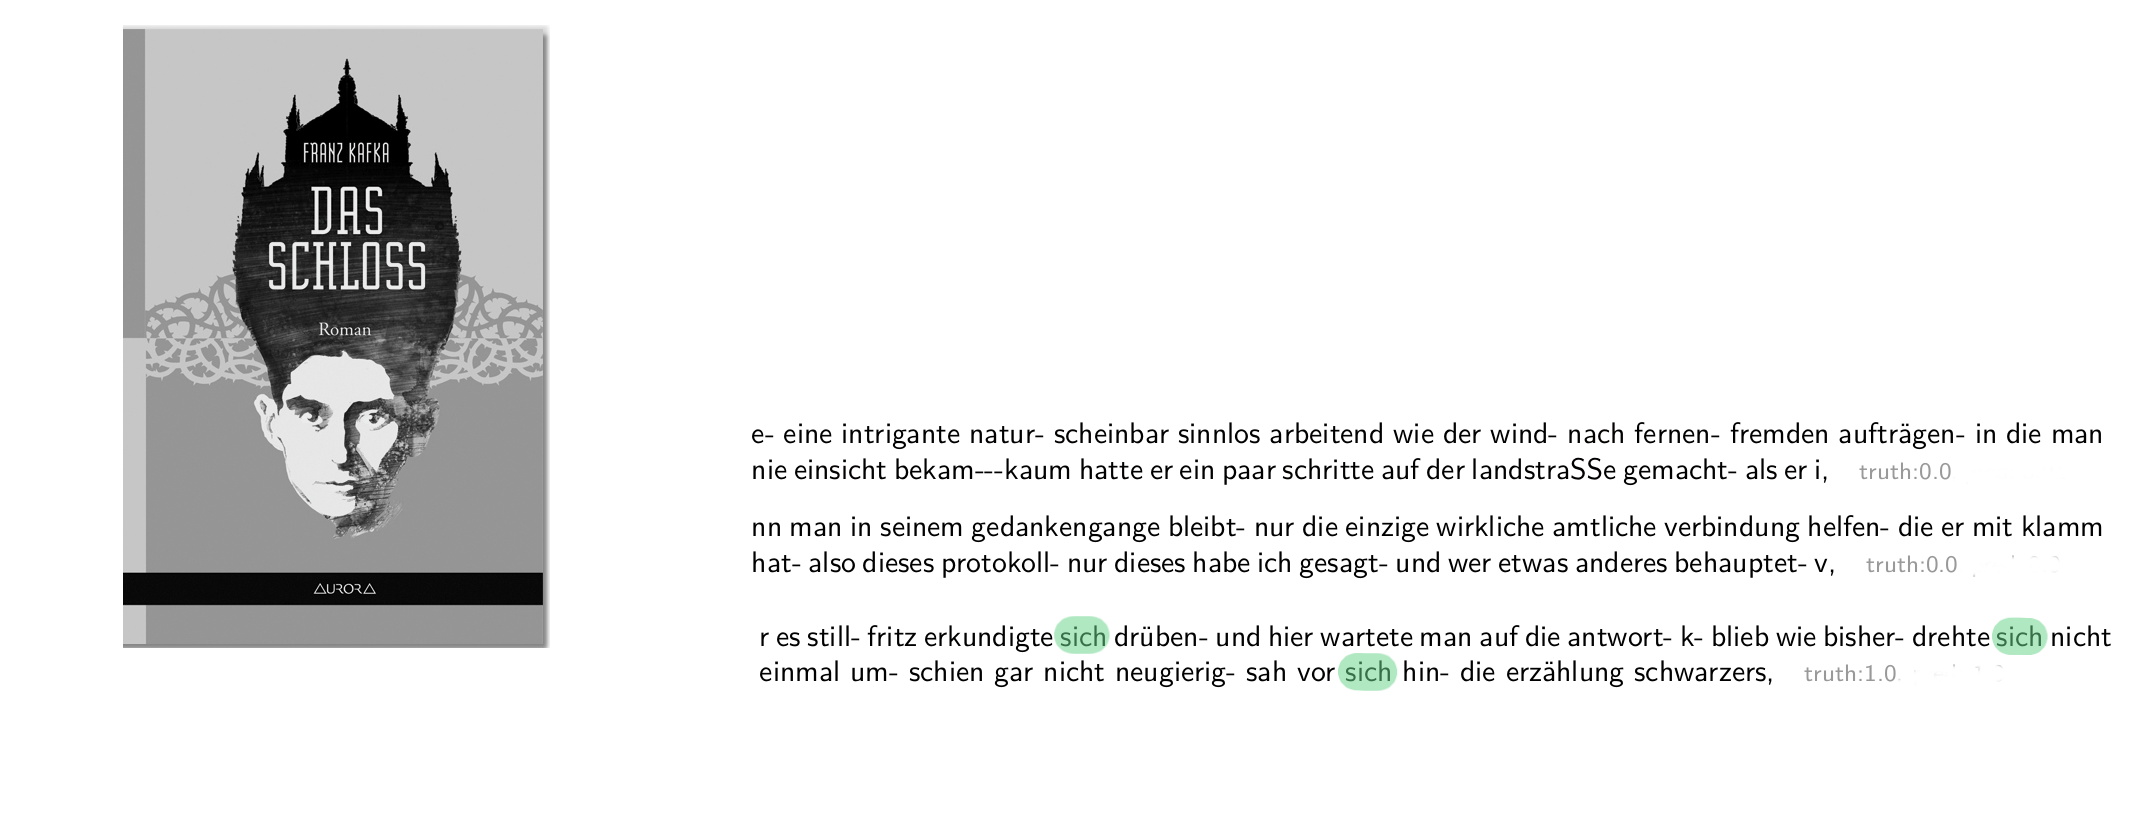
\includegraphics[width=1\textwidth]{Figures/kafkaextract1.png}
\begin{itemize}
\item extract 'sentences' \gr{(200 letters each)} and match pattern with reegex
\end{itemize}
\end{minipage}
}
\end{frame}


\begin{frame}{project structure} 
\linespread{1}\large{
\begin{minipage}{0.3\textwidth}
\raisebox{-1cm}{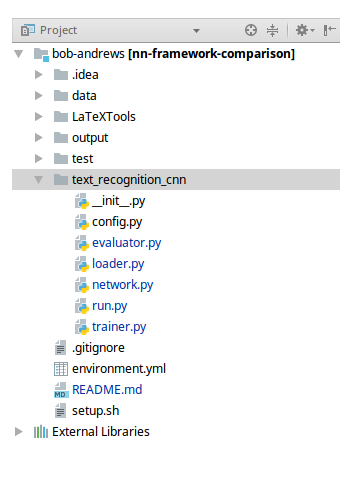
\includegraphics[width=1\textwidth]{Figures/projectstructure.png}}
\begin{tikzpicture}[overlay] 
\uncover<1->{
  \draw[draw=springgreen, line width=0.06cm,->]  
  (1.65\textwidth, 1.45\textwidth) 
  -- 
  (0.40\textwidth,0.60\textwidth); 
  }
\uncover<1->{
  \draw[draw=springgreen, line width=0.06cm,->]  
  (1.65\textwidth, 0.85\textwidth) 
  -- 
  (0.40\textwidth,0.54\textwidth); 
  }
\uncover<1->{
  \draw[draw=springgreen, line width=0.06cm,->]  
  (1.25\textwidth, 0.45\textwidth) 
  -- 
  (0.40\textwidth,0.42\textwidth); 
  }
\end{tikzpicture} 
\end{minipage}
\begin{minipage}{0.69\textwidth}

\eqc{
\begin{align}
\raisebox{-1cm}{
\includegraphics[width=2.2cm]{Figures/speechbubble.jpg}}
\quad&\RA
{\bm x}, 
{\bm y_{\rm truth}}
\notag
\end{align}
}
\eqc{
\begin{align}
n\left(w, {\bm x}\right)
\quad&\RA
{\bm y}
\notag
\end{align}
}
\eqc{
\begin{align}
{\rm loss}\left(
n\left(w, {\bm x}\right), 
{\bm y_{\rm truth}}
\right)
\quad&\RA
\left.
w
\right|_{\rm @ min}
\notag
\end{align}
}
\vspace{0.0cm}
\begin{center}
\uncover<1->{
\includegraphics[width=0.6\textwidth]{Figures/phase3.png}}
\end{center}

\end{minipage}
}
\end{frame} 

\begin{frame}{standard convolution examples}
%\animategraphics[loop,autoplay]{12}​{frame-}{0}{3}
\begin{columns}[T]%beamer
\column{0.5\textwidth}
No padding, no strides

\animategraphics[loop,autoplay, width=0.5\textwidth]{1}{Figures/no_padding_no_strides/frame-}{0}{3}

Arbitrary padding, no strides

\animategraphics[loop,autoplay, width=0.5\textwidth]{1}{Figures/arbitrary_padding_no_strides/frame-}{0}{35}

% gifsicle --unoptimize no_padding_no_strides.gif | convert - frame-%d.png
 

\column{0.5\textwidth}
No padding but strides

\animategraphics[loop,autoplay, width=0.5\textwidth]{1}{Figures/no_padding_strides/frame-}{0}{3}

padding and strides

\animategraphics[loop,autoplay, width=0.5\textwidth]{1}{Figures/padding_strides/frame-}{0}{8}

% gifsicle --unoptimize no_padding_no_strides.gif | convert - frame-%d.png
\end{columns}


\citeWork{https://github.com/vdumoulin/conv\textunderscore arithmetic} \citeWork{ thx Philipp}
%\animategraphics[loop,autoplay]{6}‌​{frame-}{0}{3}
%\animategraphics[loop,autoplay]{12}{Figures/layersexplained}{0}{1}
%\includemovie{1cm}{1cm}{Figures/no_padding_no_strides.gif}
\end{frame}


\begin{frame}{convolutions example}
\linespread{1}\large{
\begin{minipage}{1\textwidth}
\only<1>{
\includegraphics[width=0.99\textwidth]{Figures/layersexplained0.png}}\only<2>{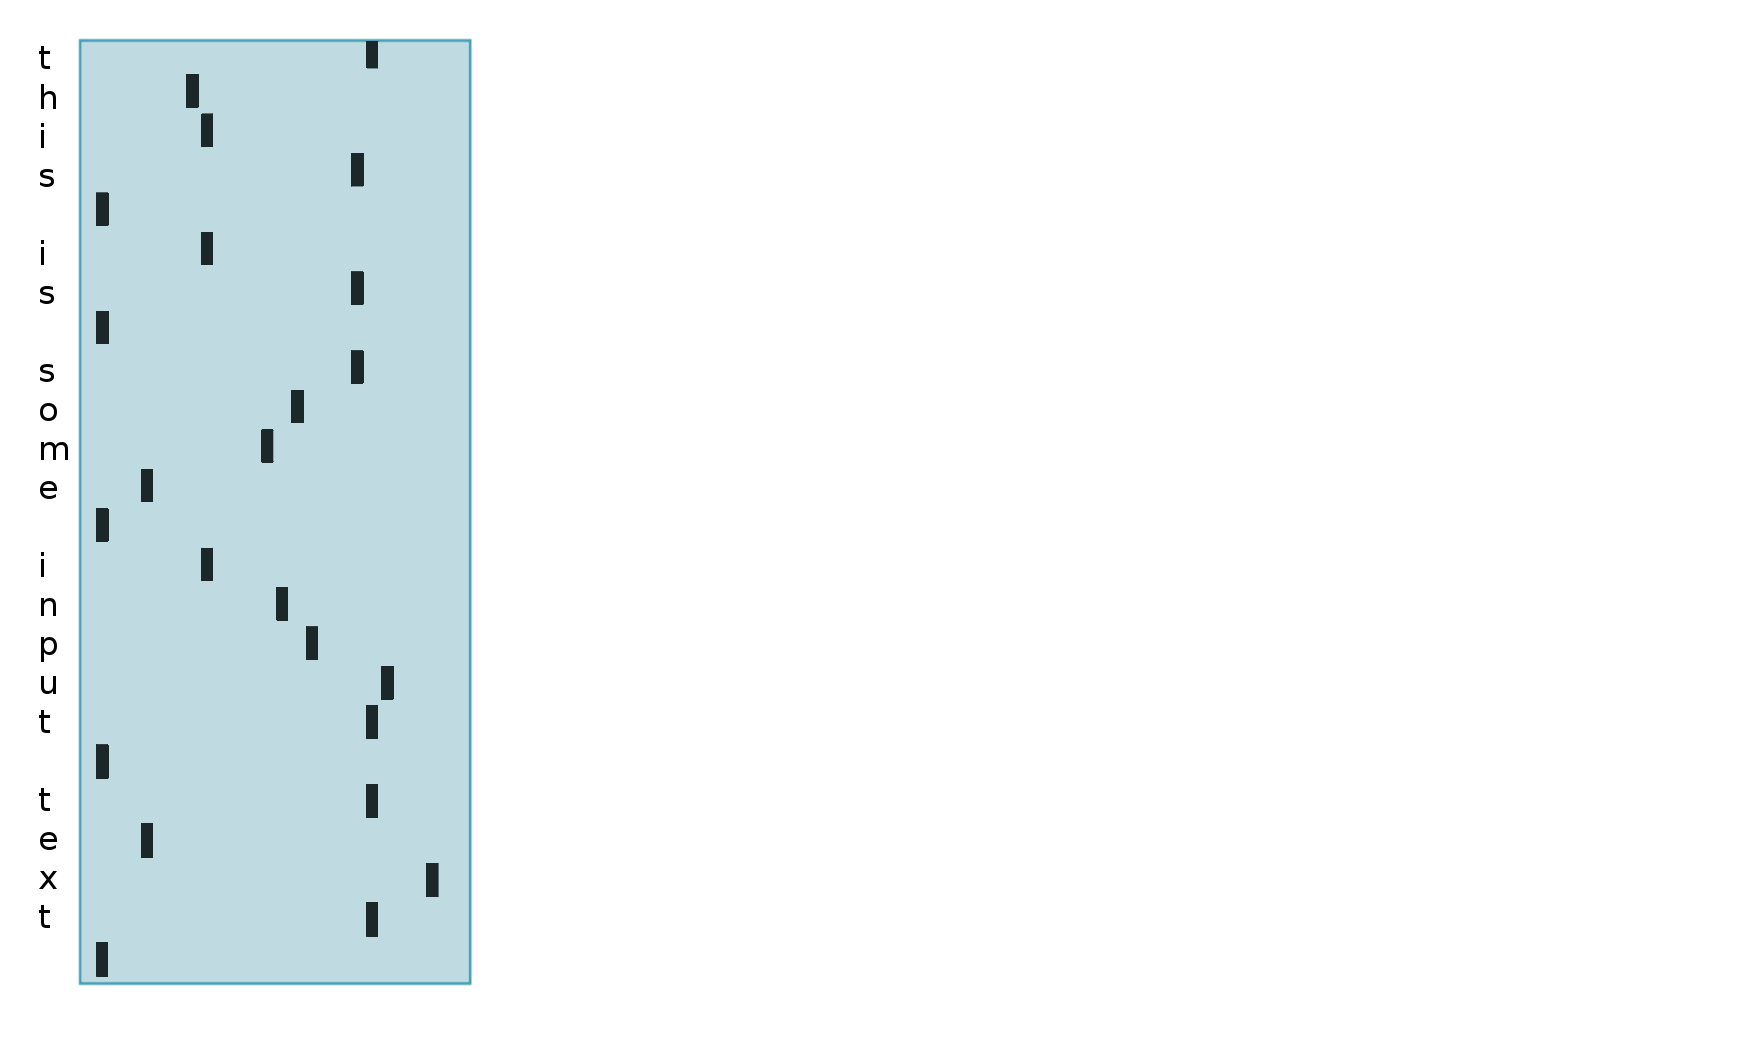
\includegraphics[width=0.99\textwidth]{Figures/layersexplained1.png}}\only<3>{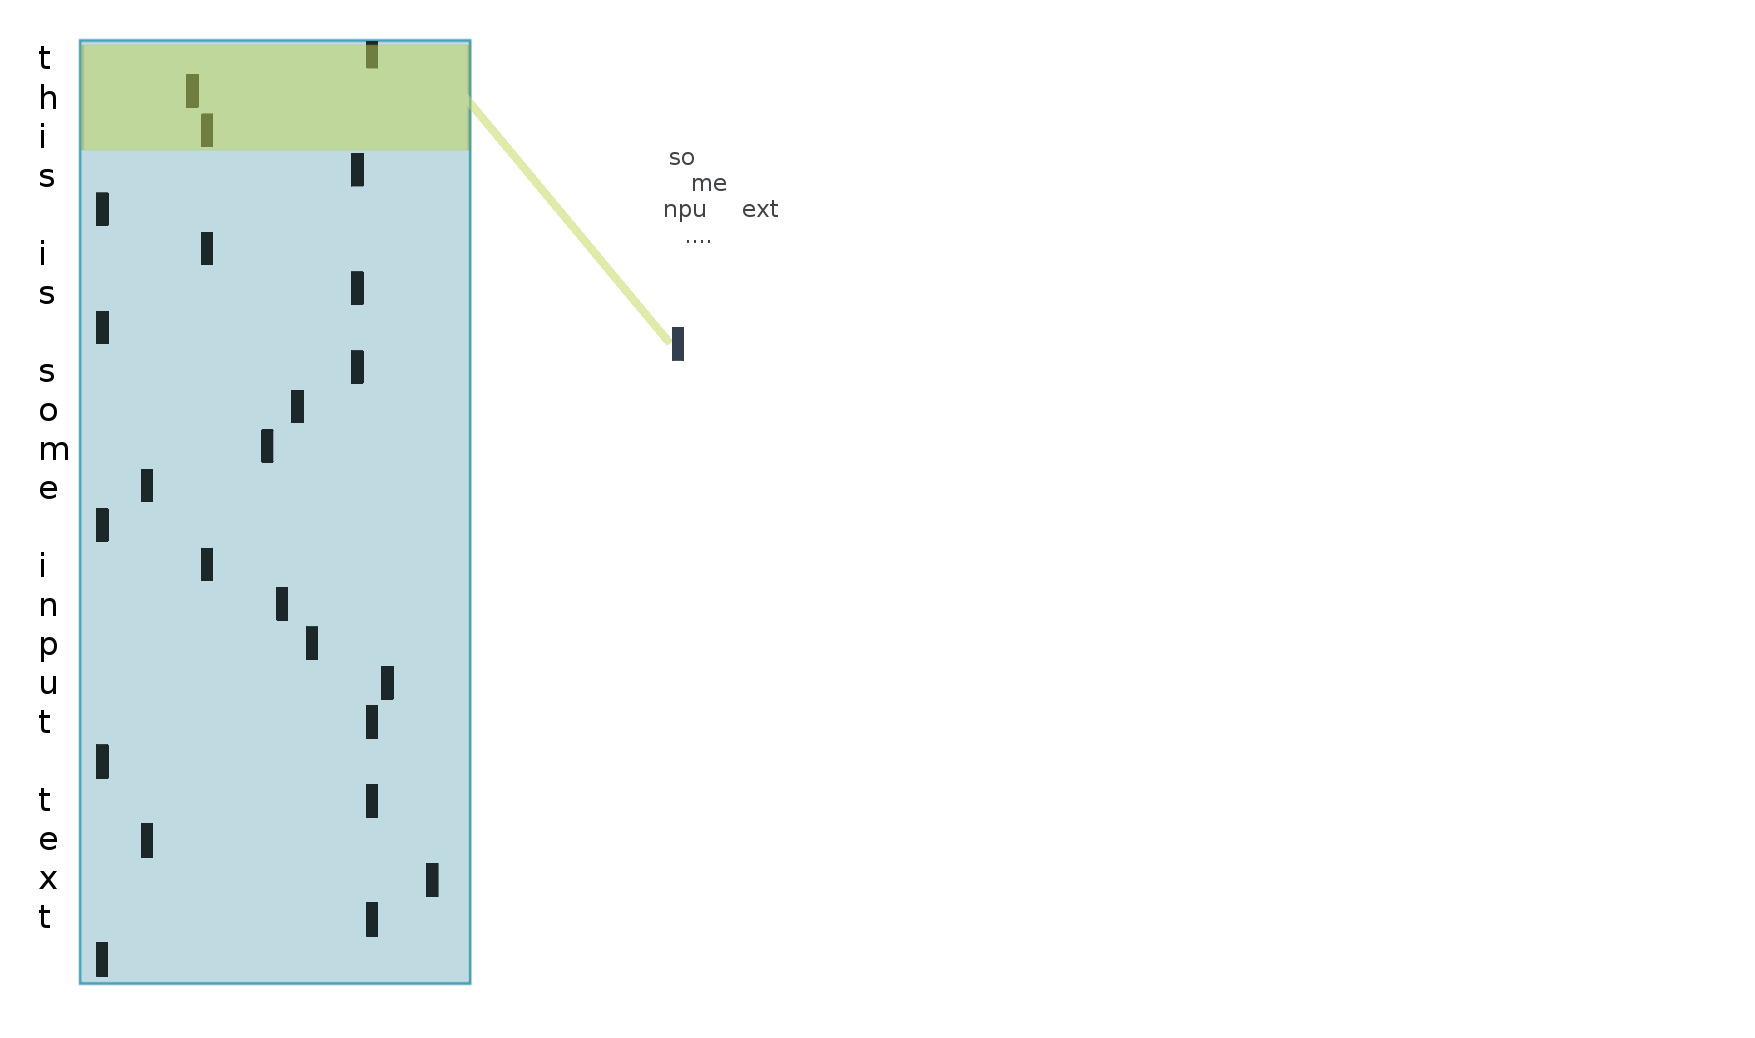
\includegraphics[width=0.99\textwidth]{Figures/layersexplained21.png}}\only<4>{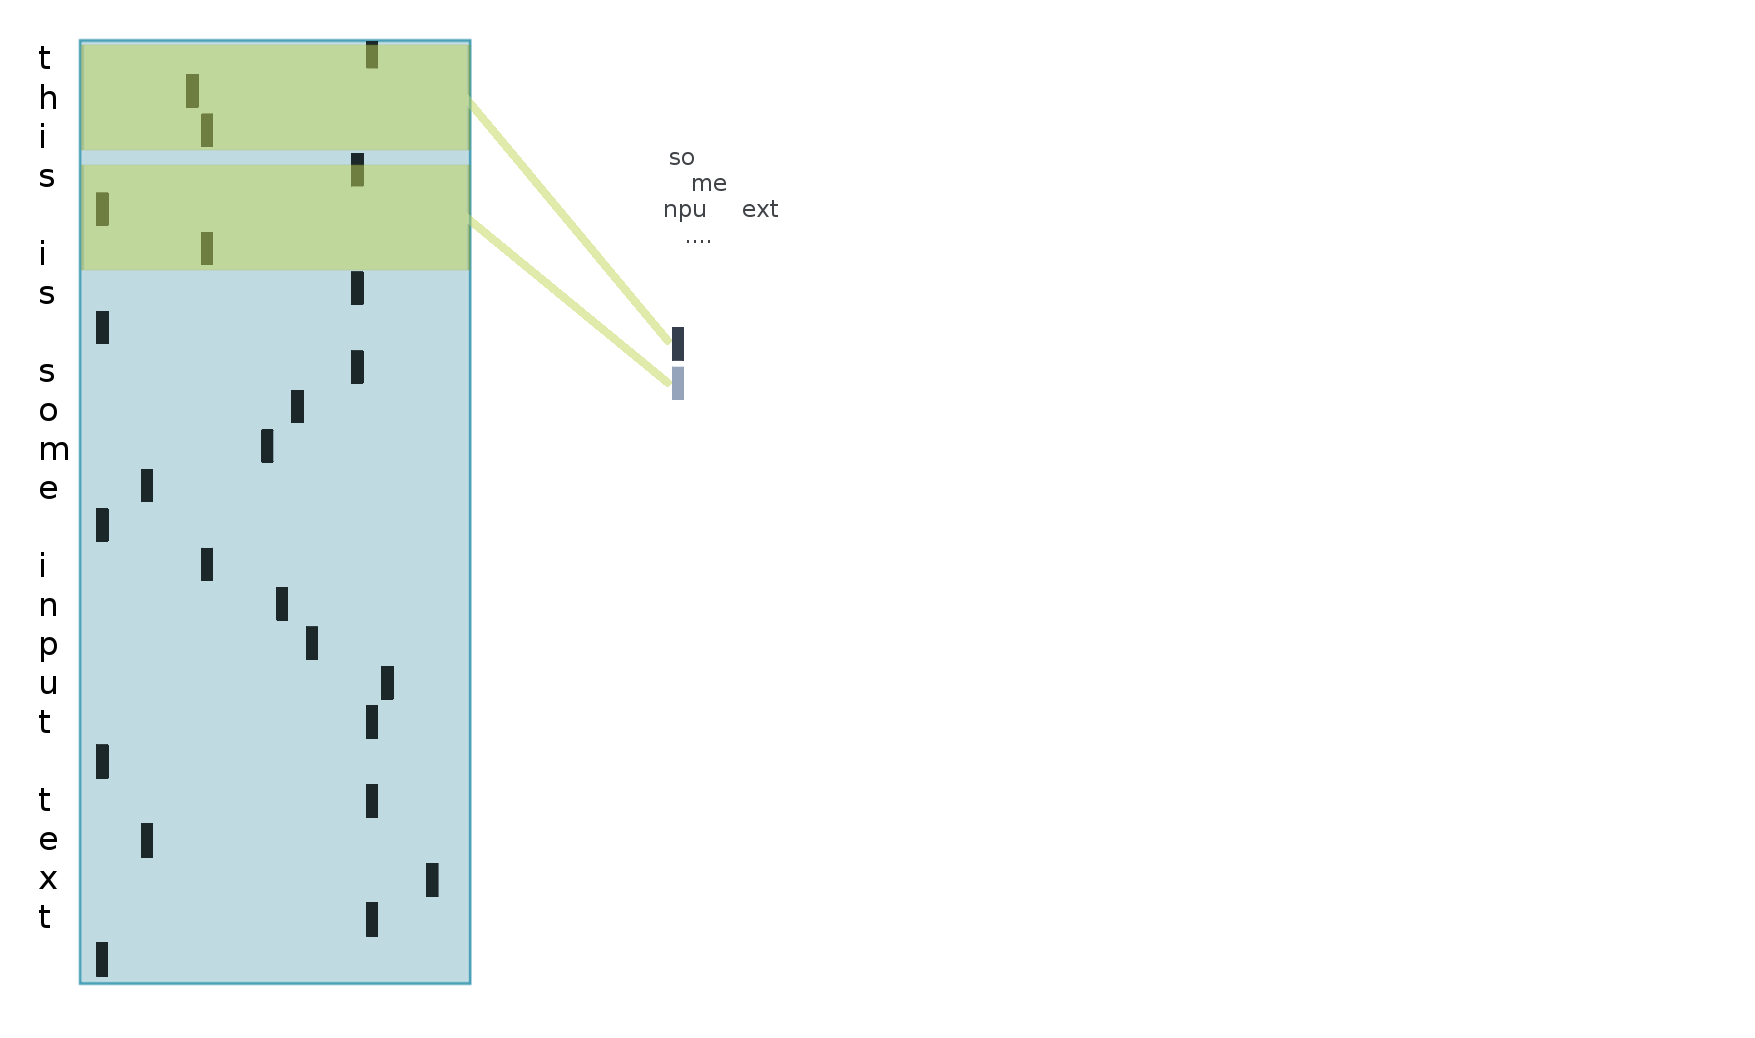
\includegraphics[width=0.99\textwidth]{Figures/layersexplained22.png}}\only<5>{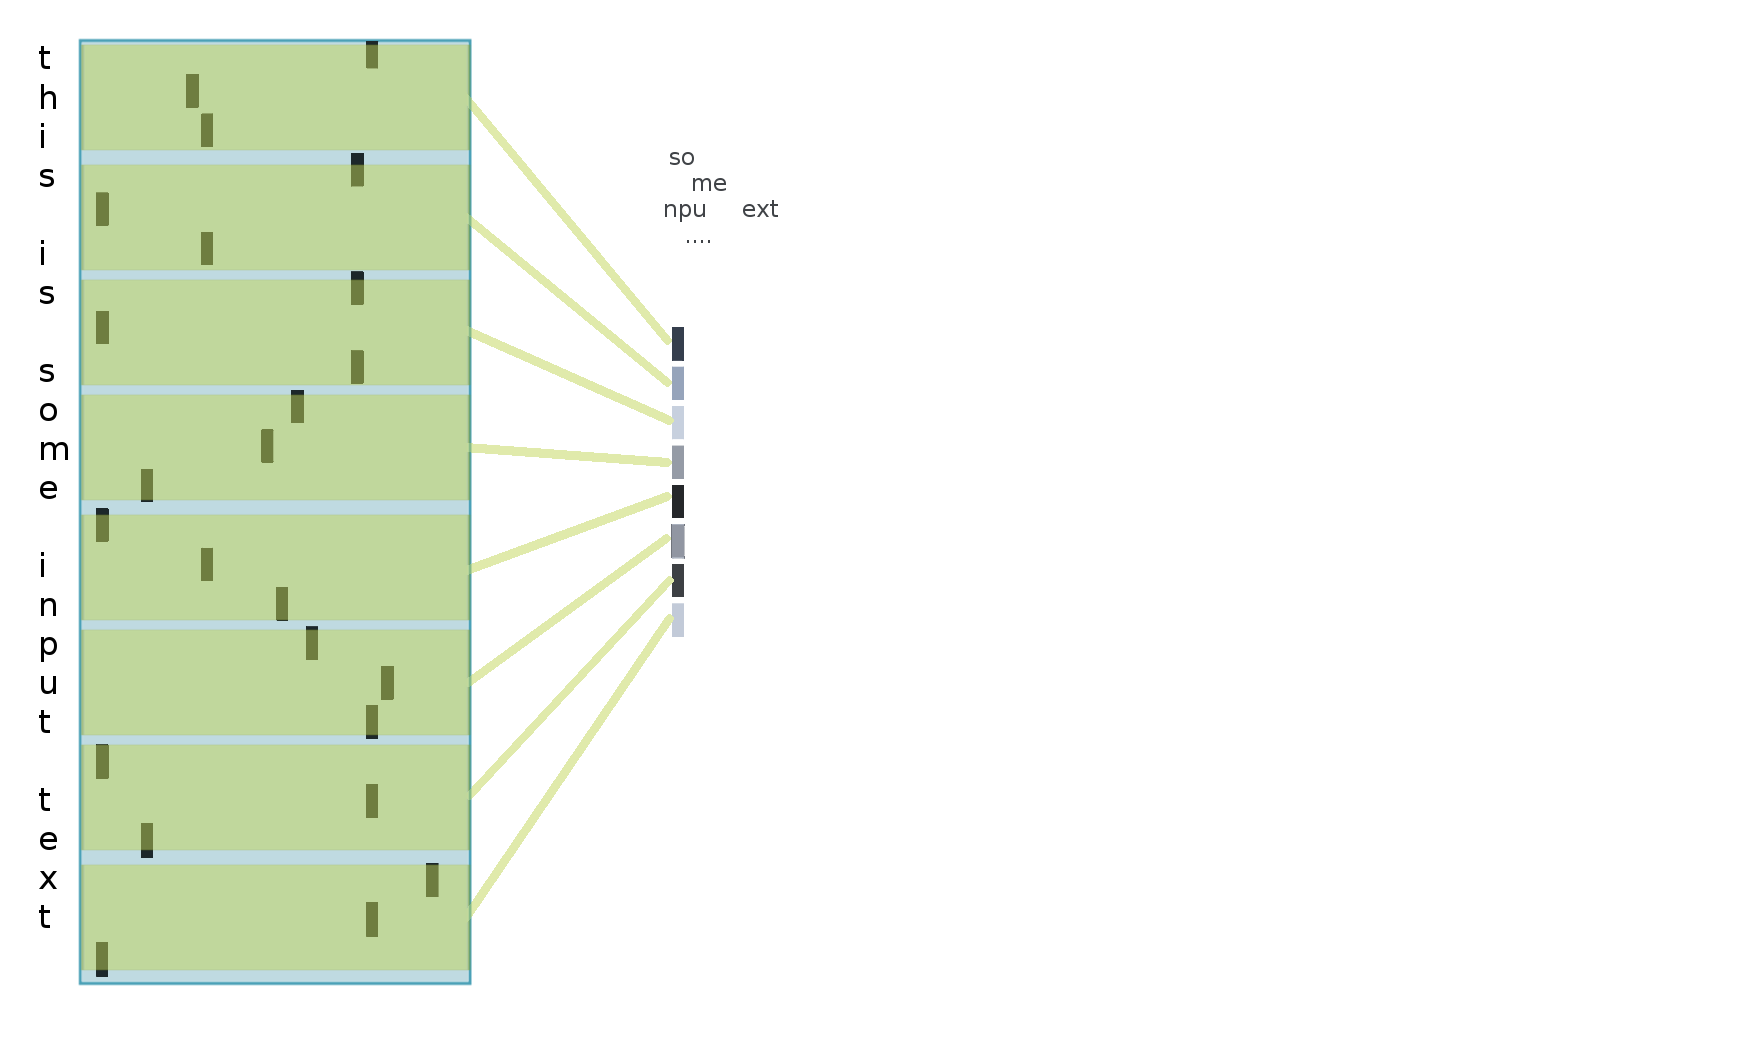
\includegraphics[width=0.99\textwidth]{Figures/layersexplained23.png}}\only<6>{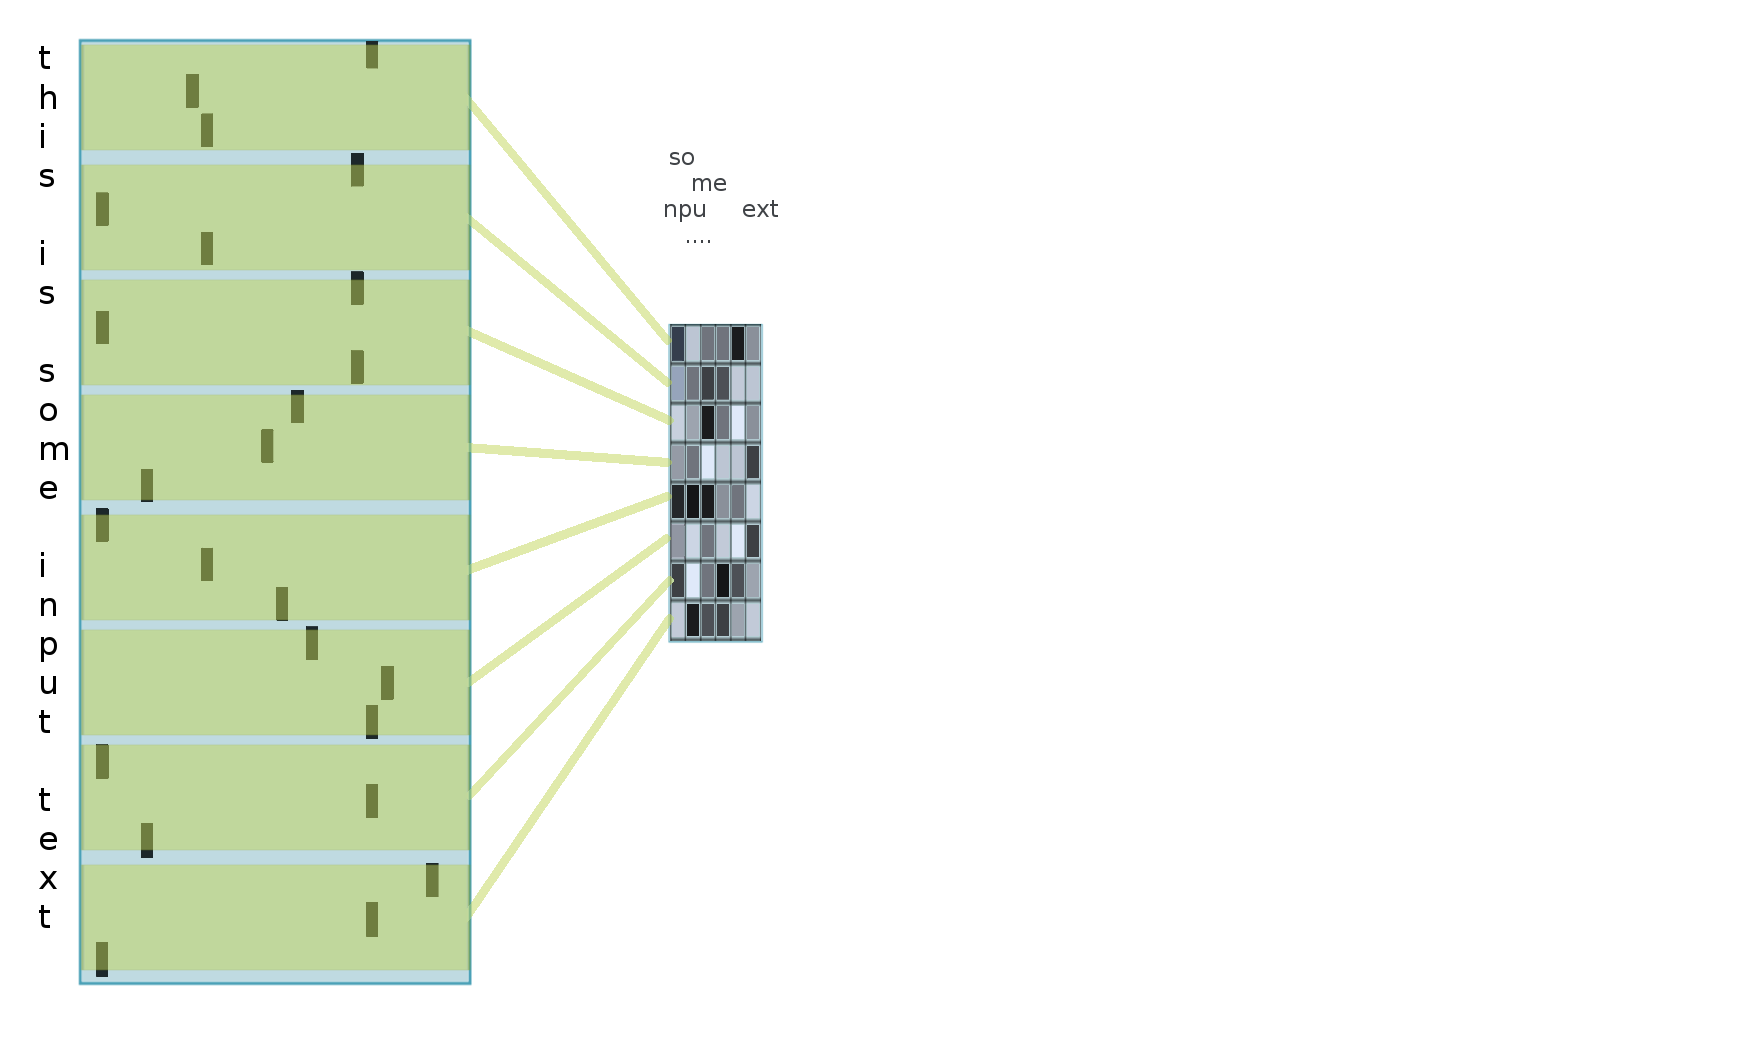
\includegraphics[width=0.99\textwidth]{Figures/layersexplained3.png}}\only<7>{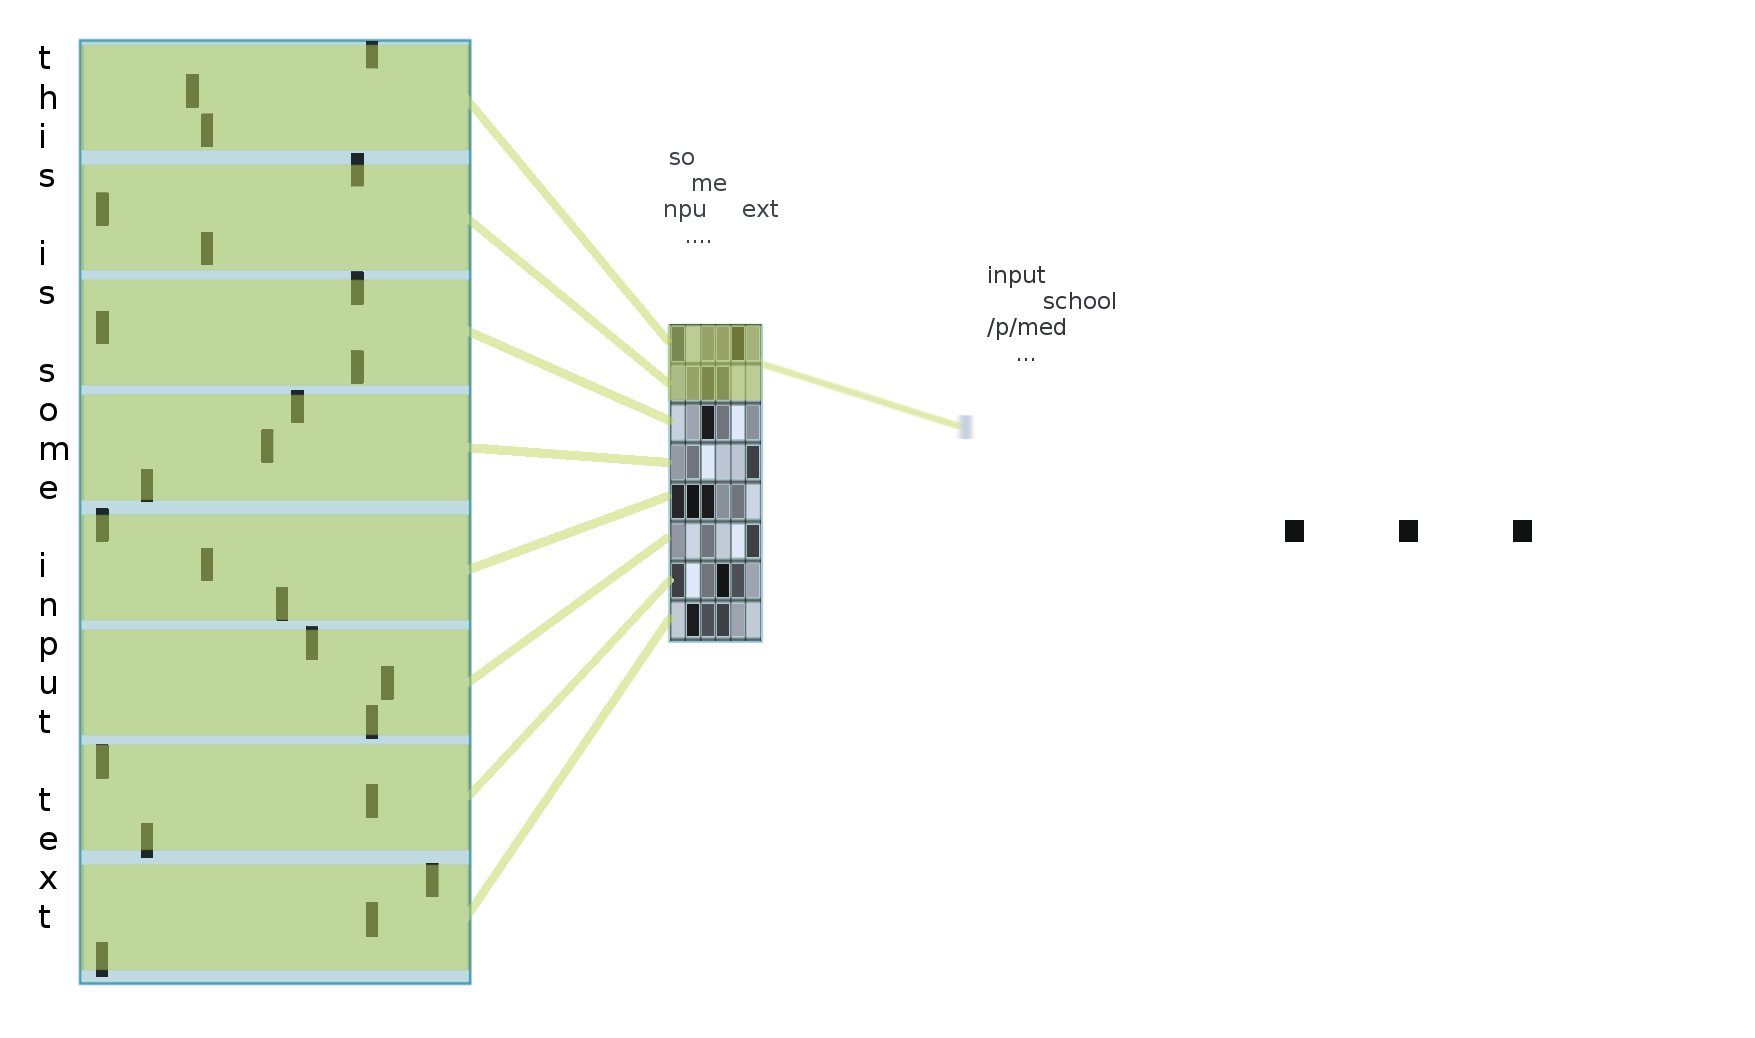
\includegraphics[width=0.99\textwidth]{Figures/layersexplained4.png}}
\end{minipage}
}
\end{frame}




\begin{frame}{network}
%{{{
\linespread{1}\large{
\begin{minipage}{1\textwidth}
\hspace{-1.1cm}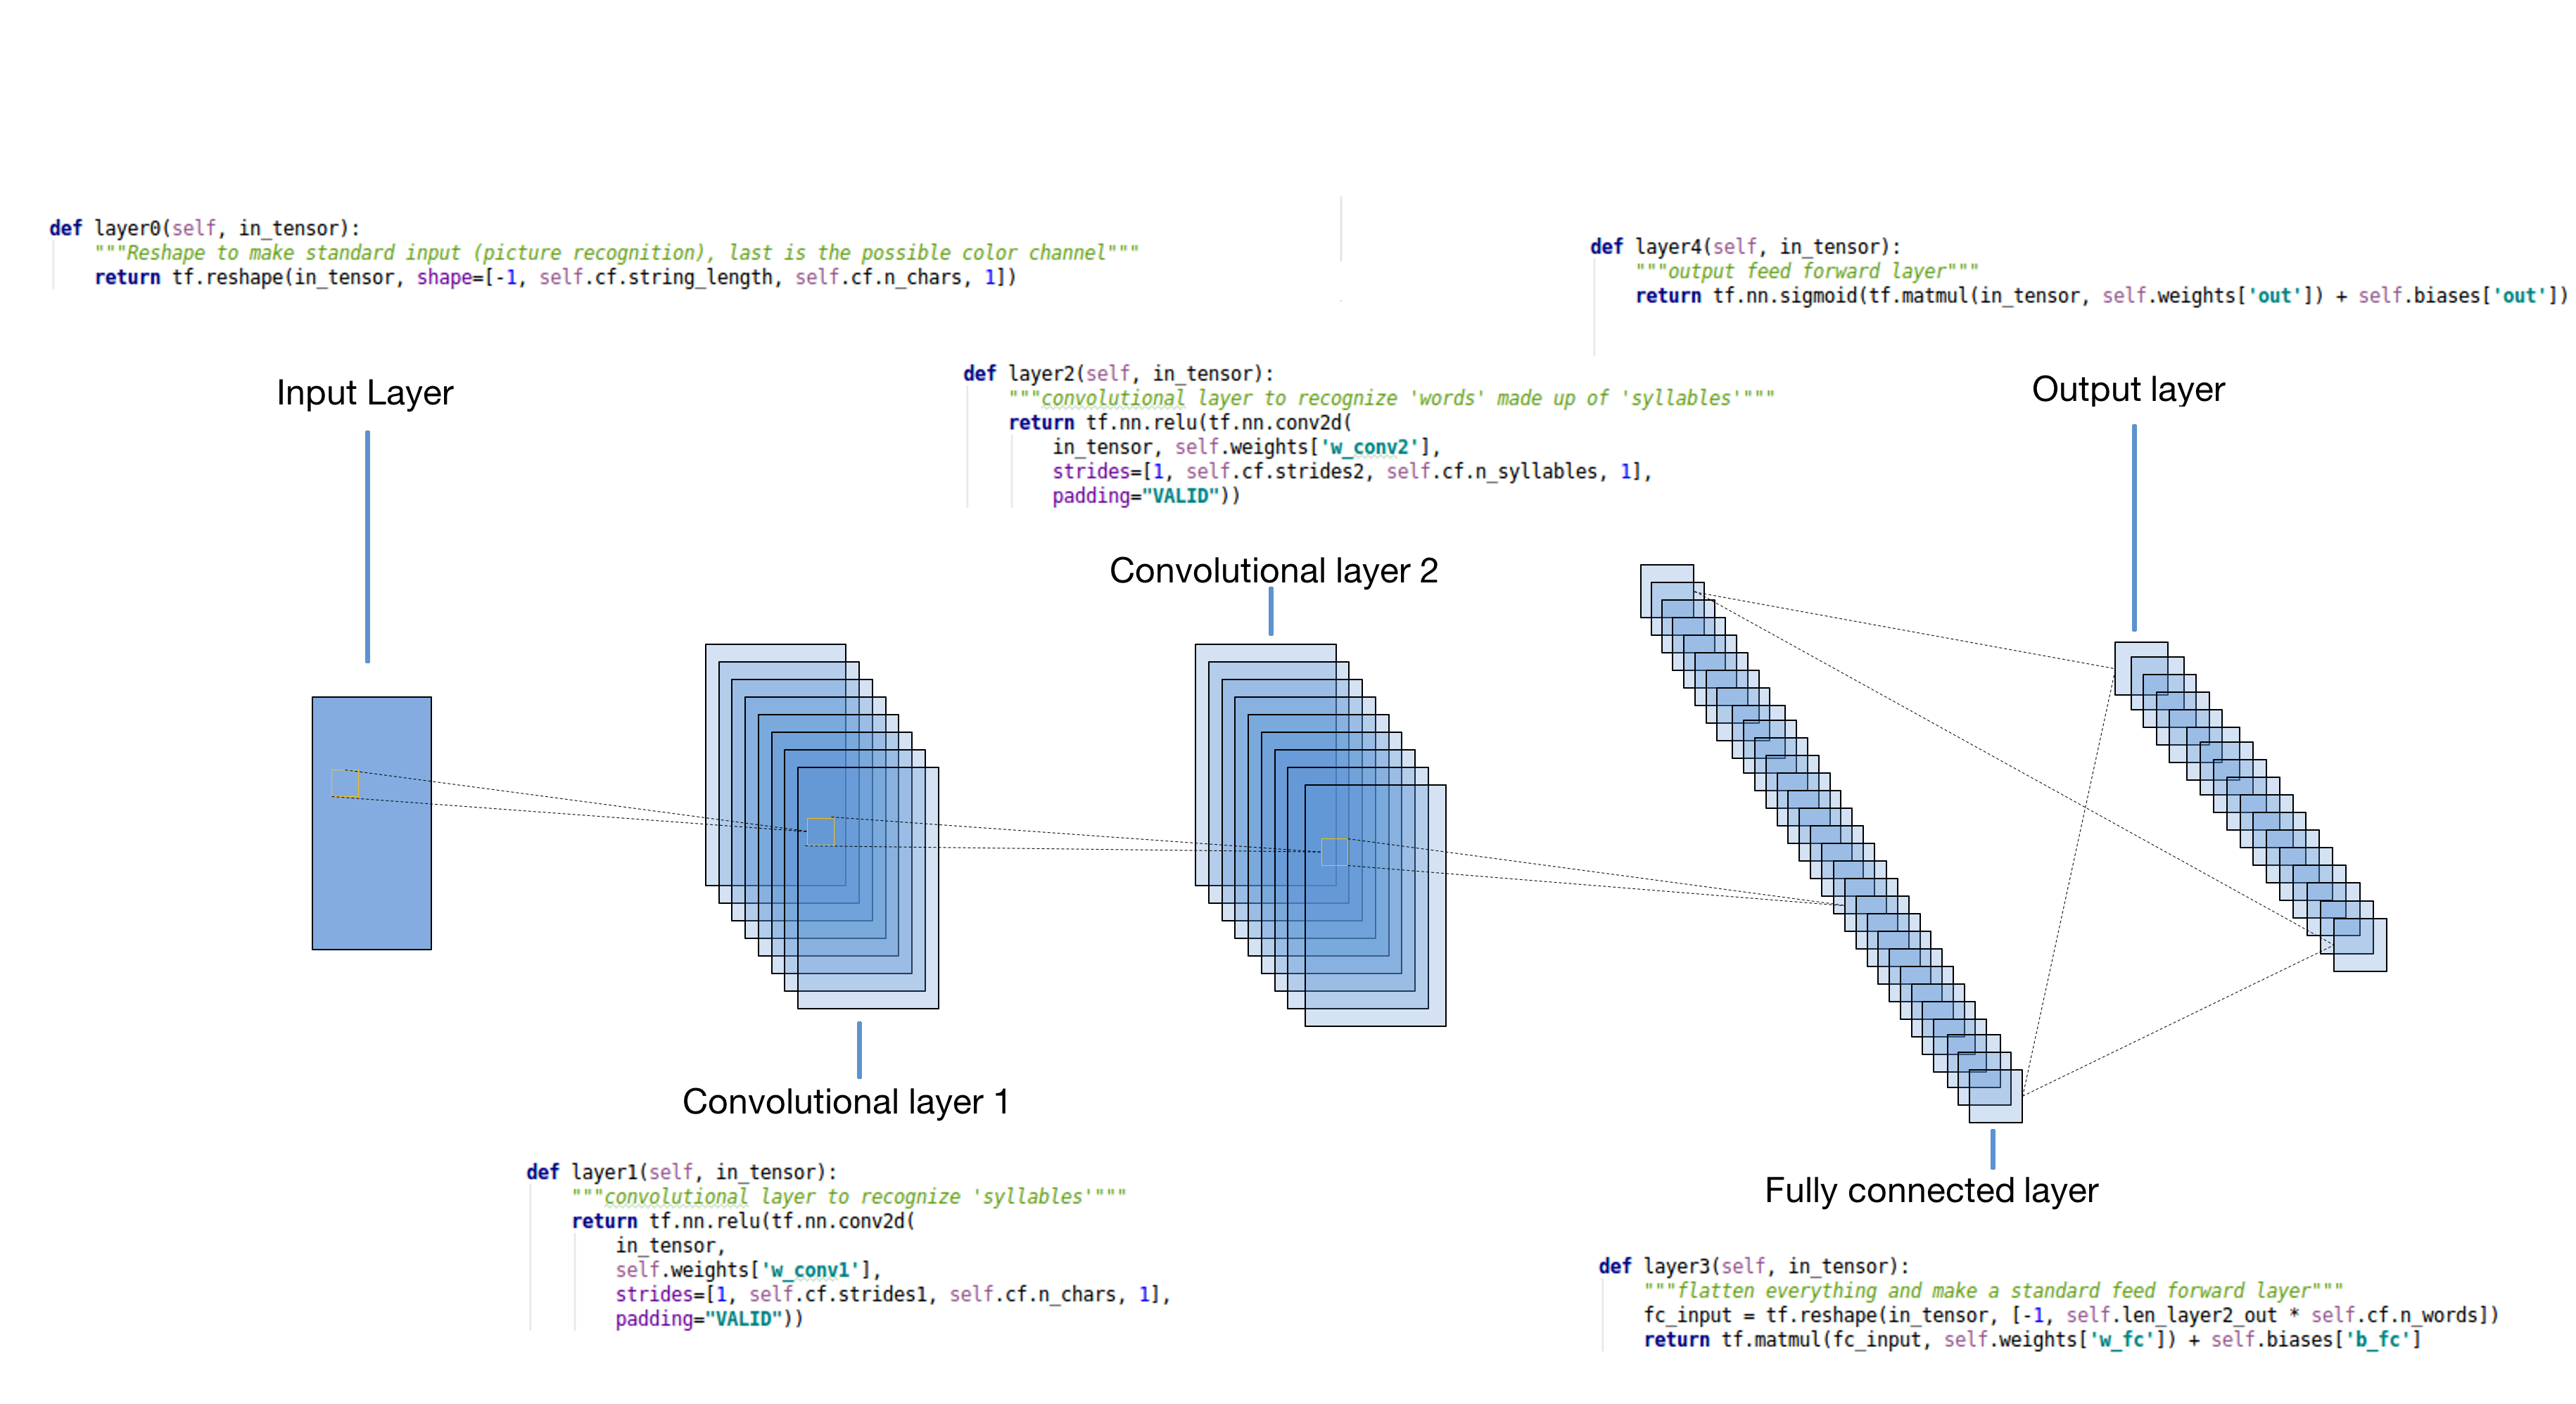
\includegraphics[width=1.1\textwidth]{Figures/cnn_architecture.png}
\end{minipage}
}
\end{frame}%}}}
 

\begin{frame}{step through code}
%{{{
\linespread{1}\small{
\begin{minipage}{0.29\textwidth}

\begin{itemize}
\uncover<1->{\item[1] datamart}
\uncover<2->{\item[2] network ini}
\uncover<4->{\item[3] graph ini}
\uncover<7->{\item[4] fitting \raisebox{-3mm}{
\includegraphics[width=0.85cm]{Figures/tensorflow_logo_big.png}}
\begin{center}
$$w_{\rm I}$$

\RB

$$w_{\rm  I} - \gamma\sum\limits_{\rm batch}\frac{\partial {\rm loss}}{\partial w_{\rm  I}}$$
\end{center}
}
\end{itemize}
\end{minipage}
\begin{minipage}{0.69\textwidth}
\only<1>{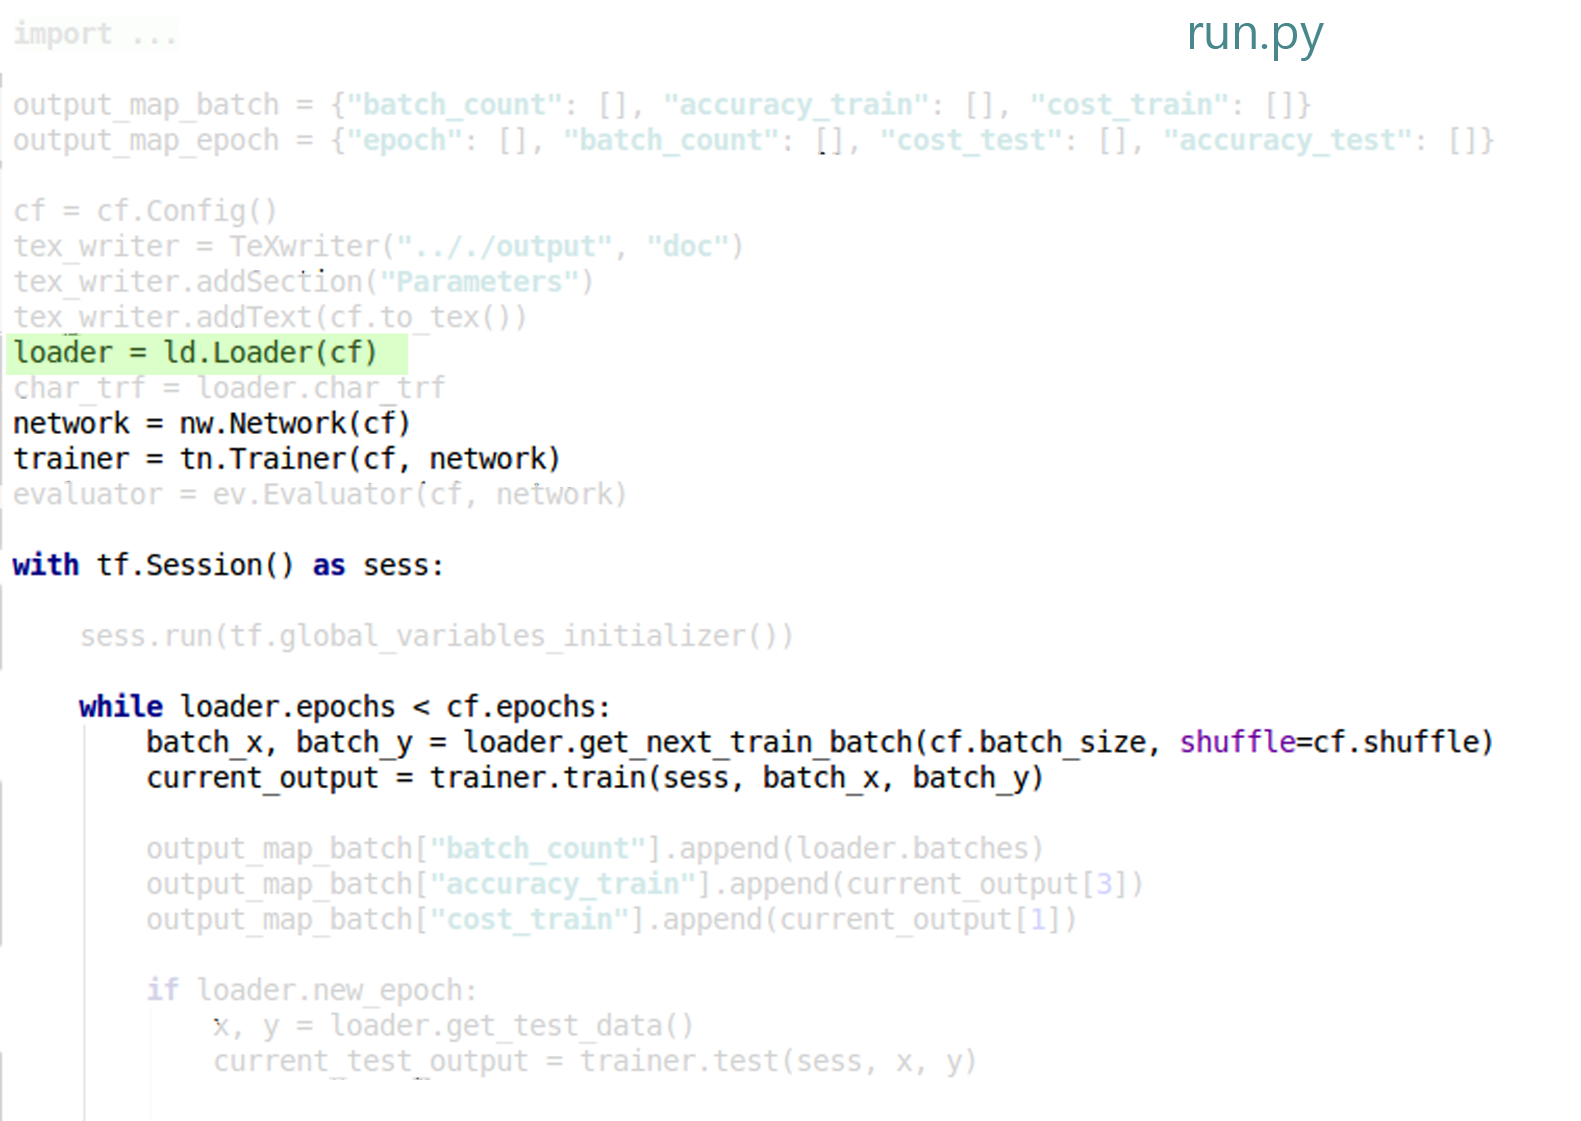
\includegraphics[width=1\textwidth]{Figures/code1_run1.png}}\only<2>{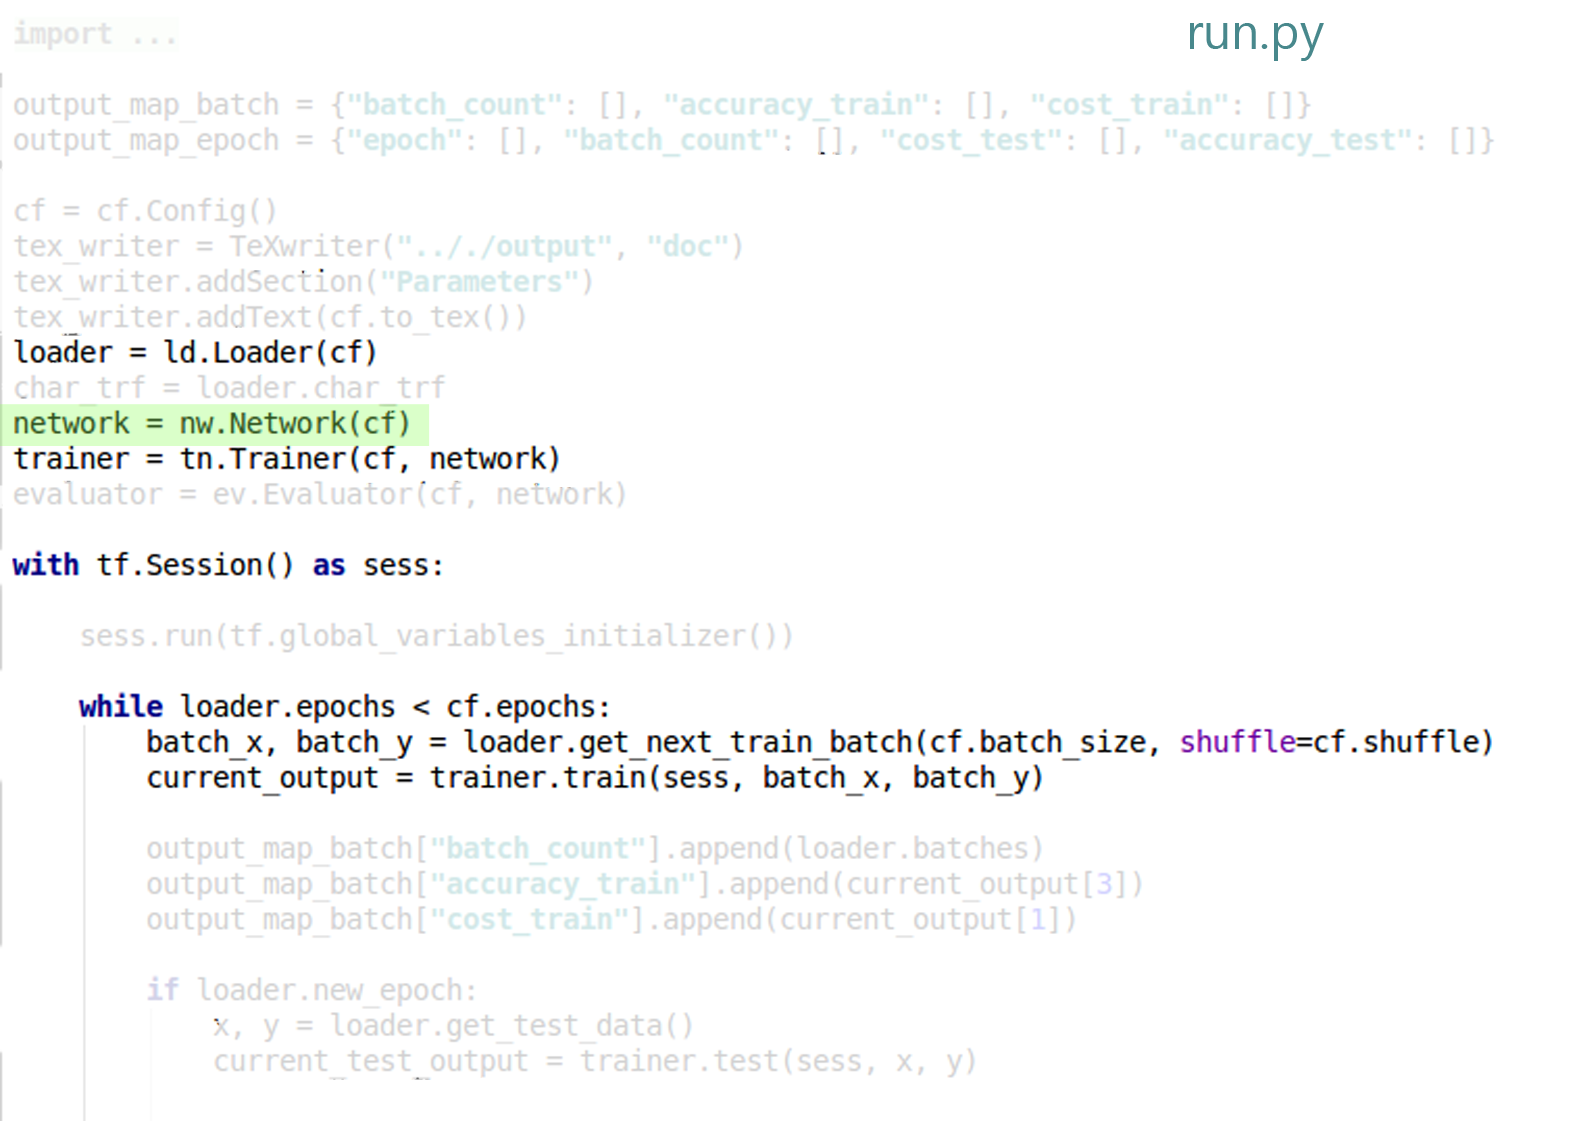
\includegraphics[width=1\textwidth]{Figures/code2_run2.png}}\only<3>{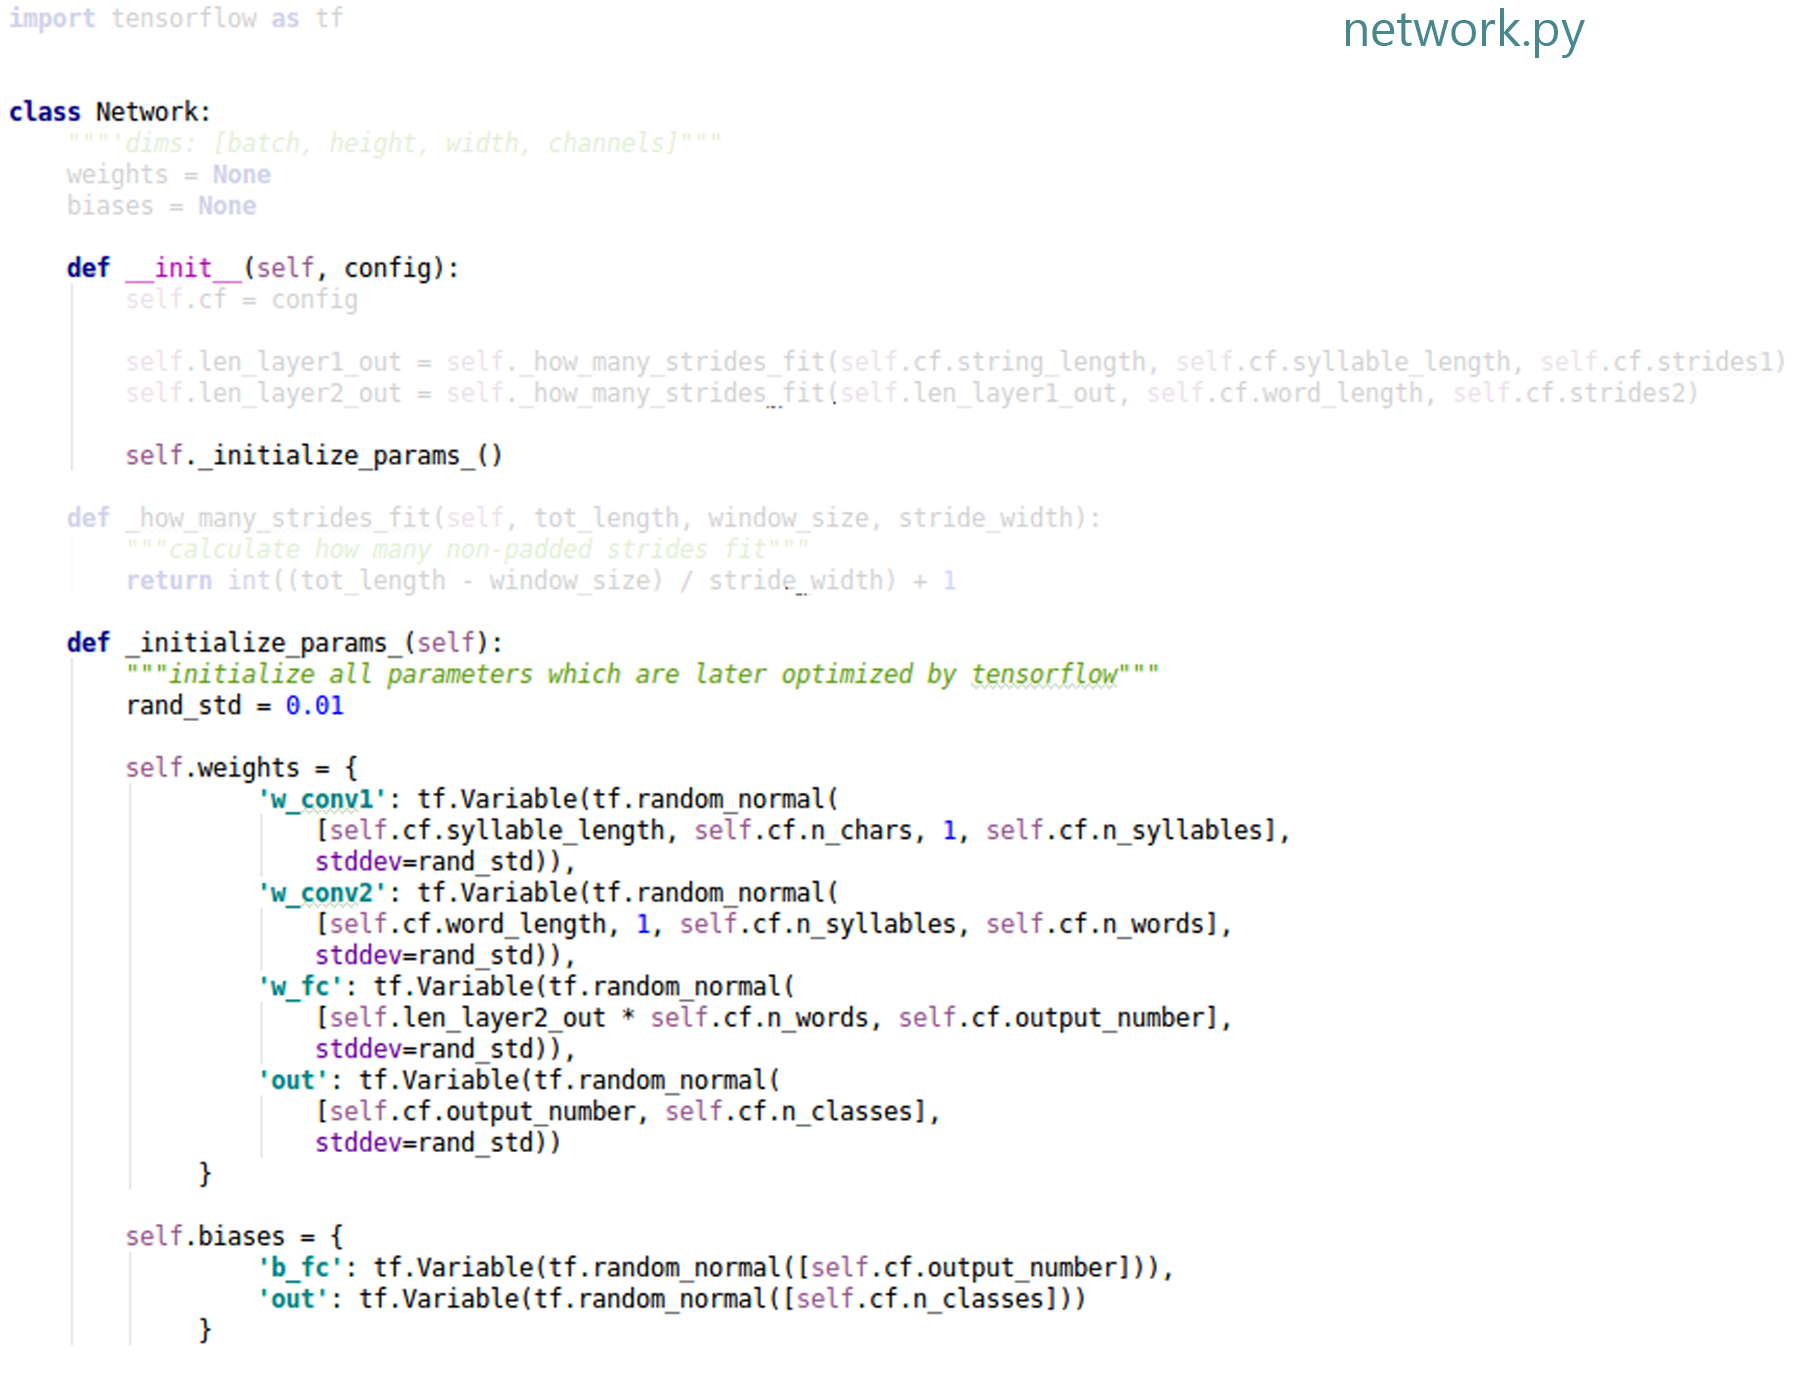
\includegraphics[width=1.2\textwidth]{Figures/code3_networkcodeinit.png}}\only<4>{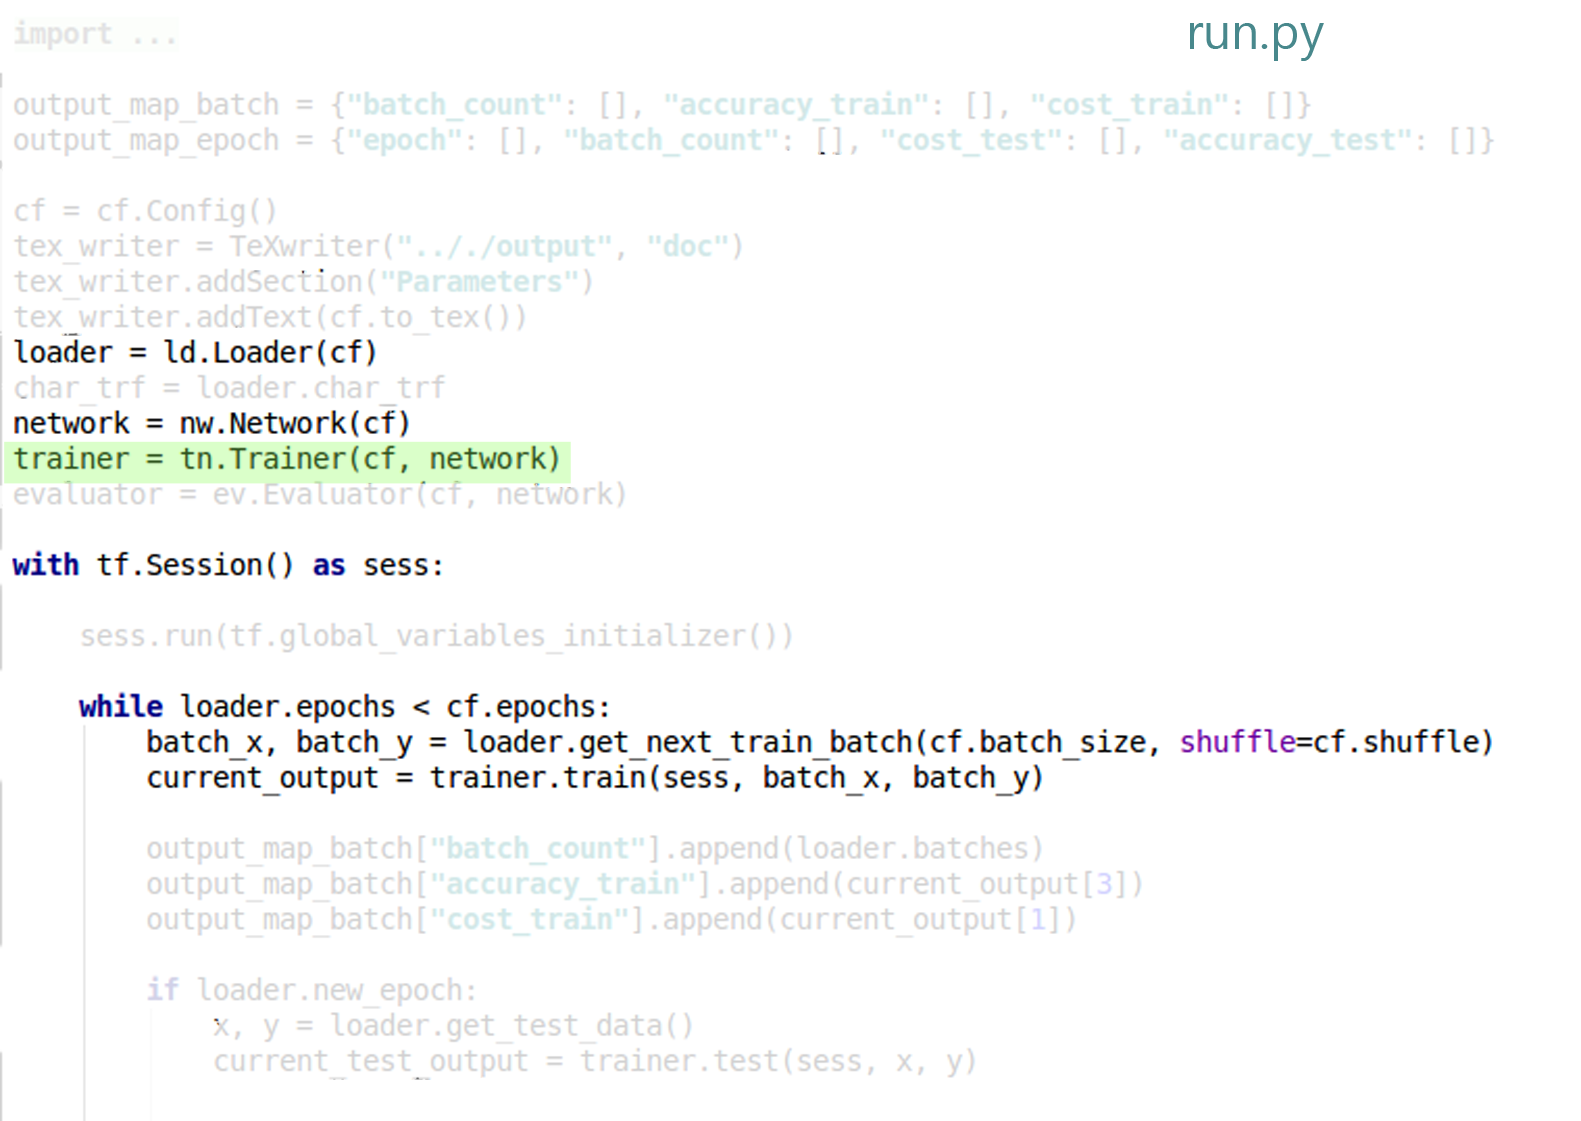
\includegraphics[width=1\textwidth]{Figures/code4_run3.png}}\only<5>{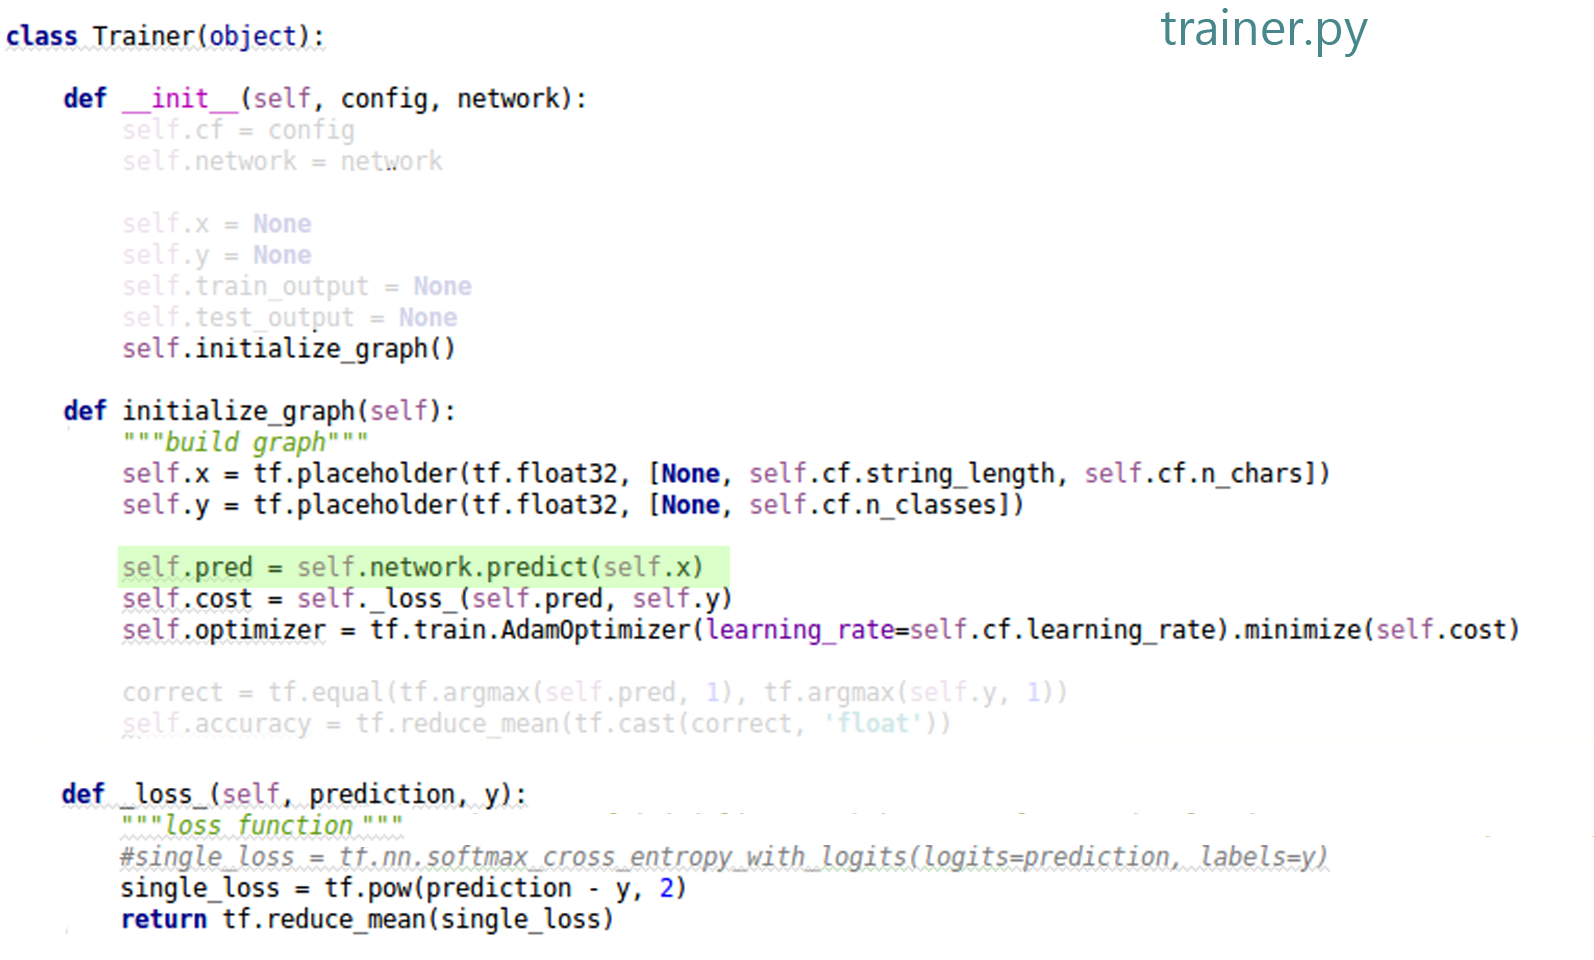
\includegraphics[width=1\textwidth]{Figures/code5_traininit.png}}\only<6>{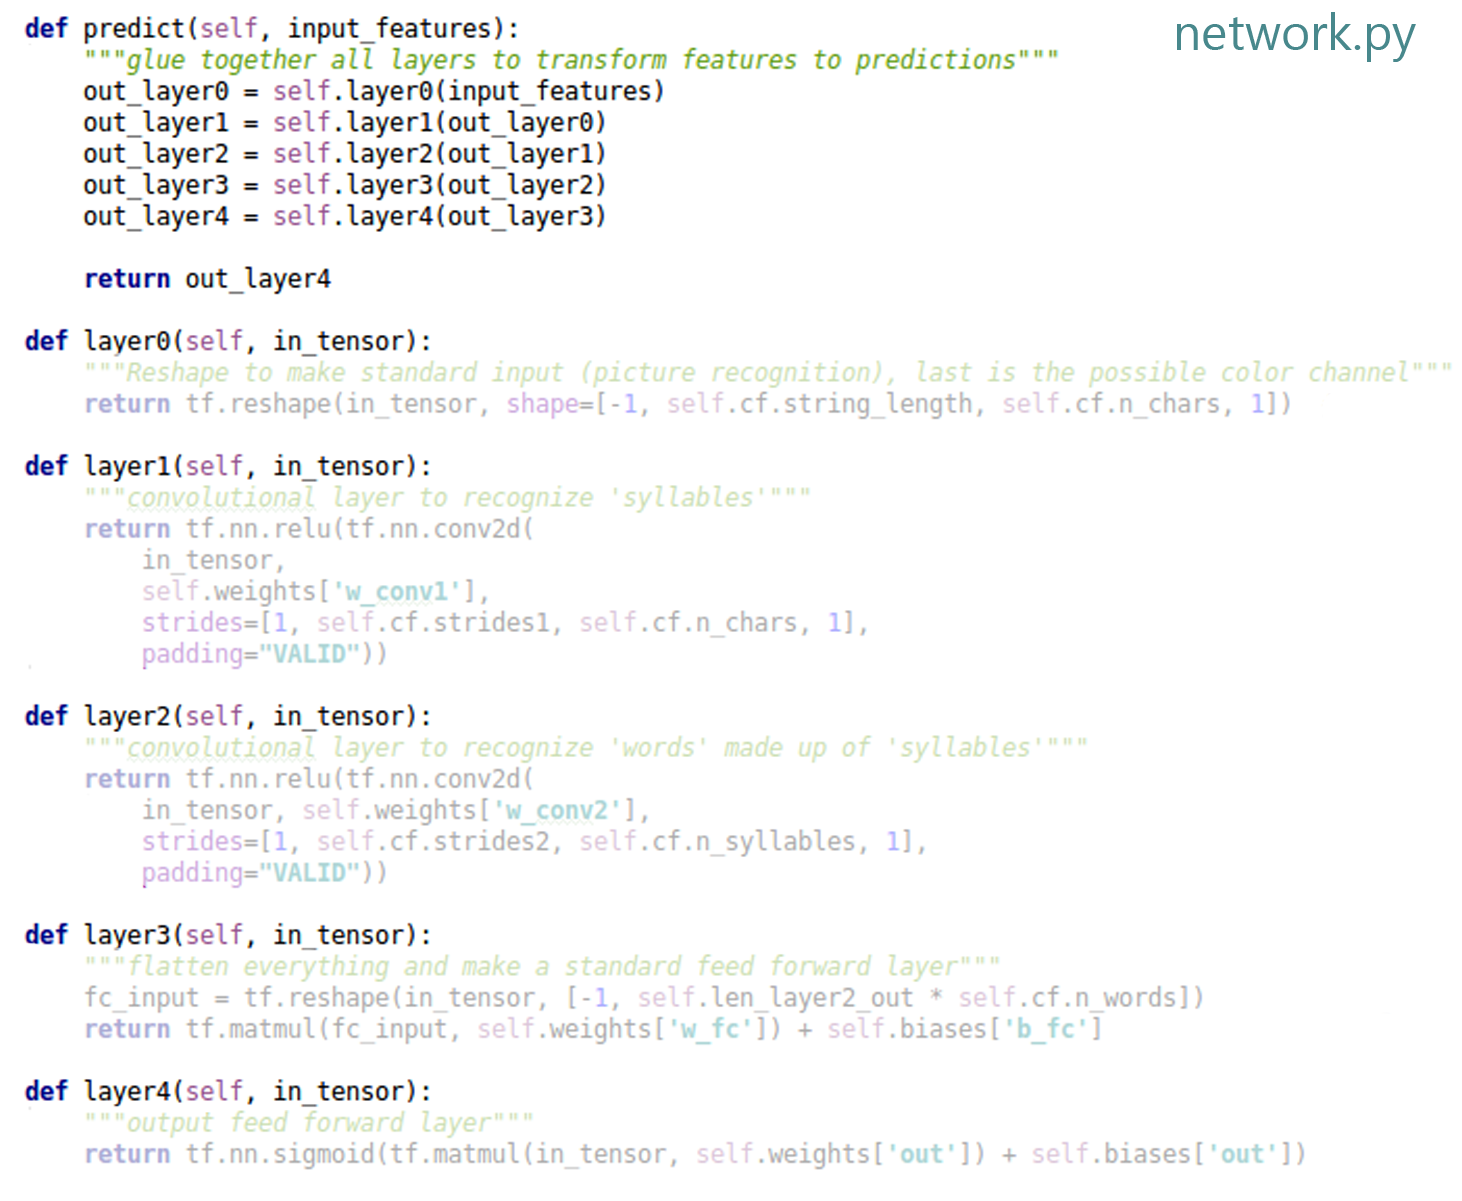
\includegraphics[width=1\textwidth]{Figures/code6_networkpredict.png}}\only<7>{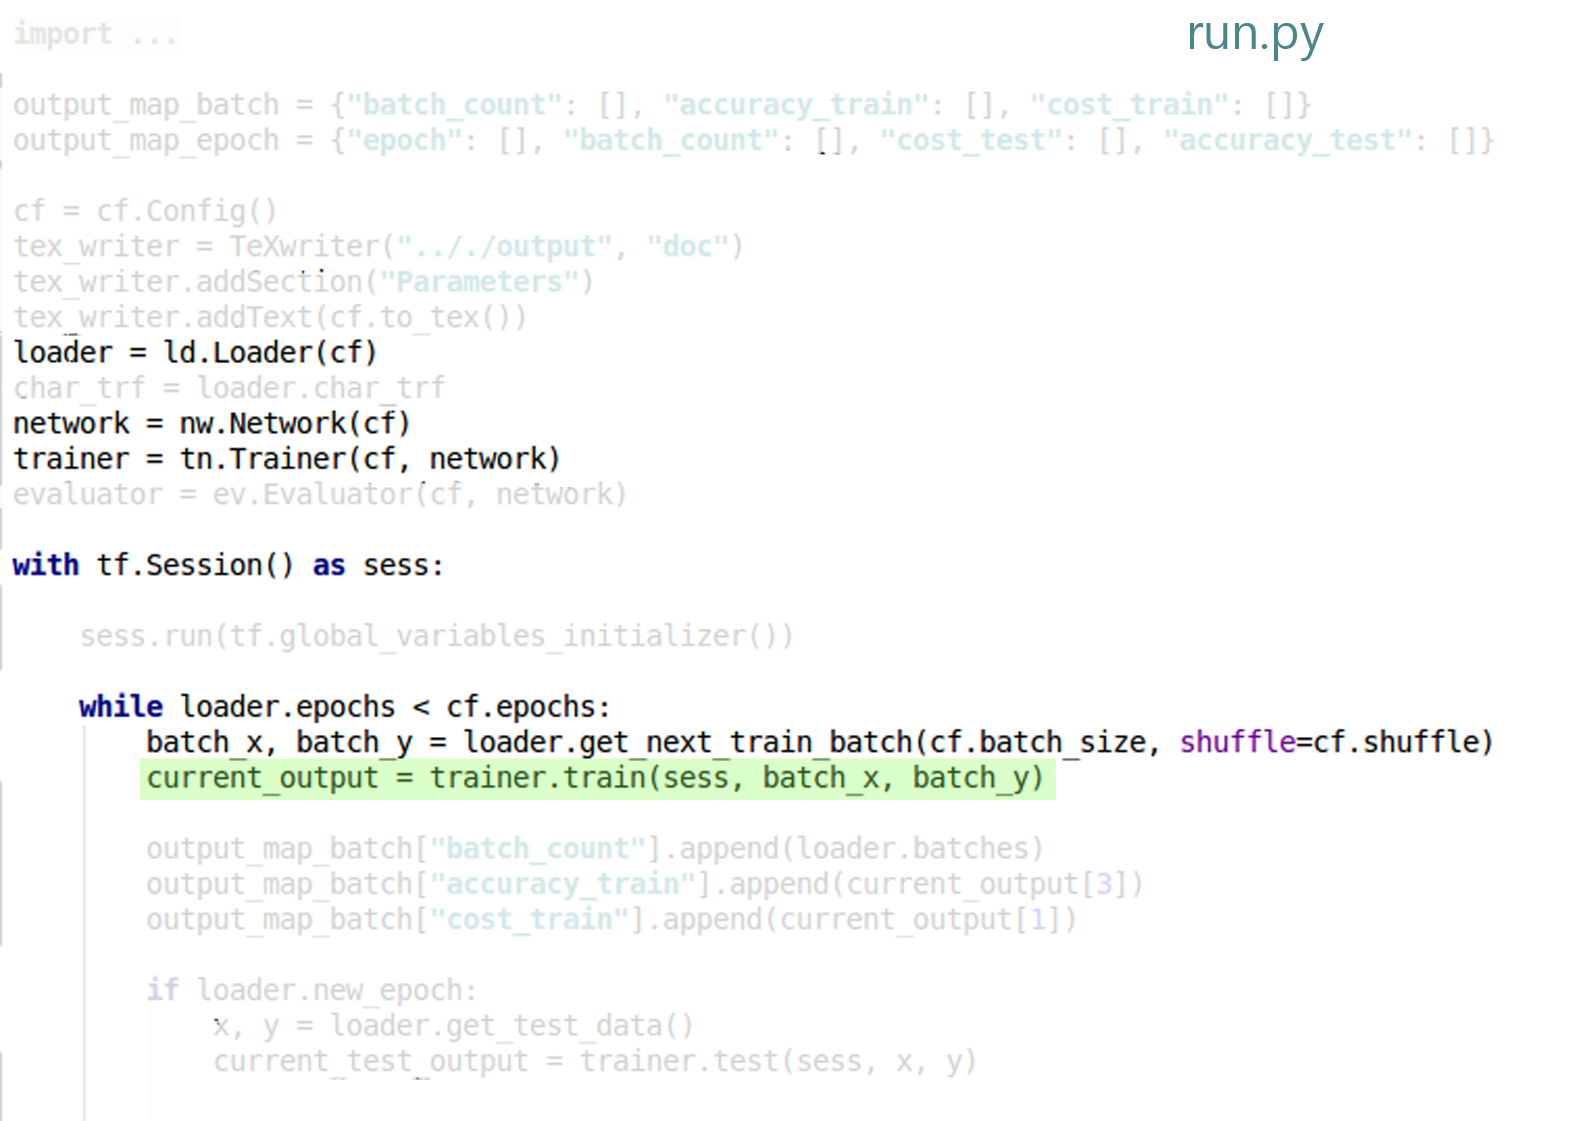
\includegraphics[width=1\textwidth]{Figures/code7_run4.png}}\only<8>{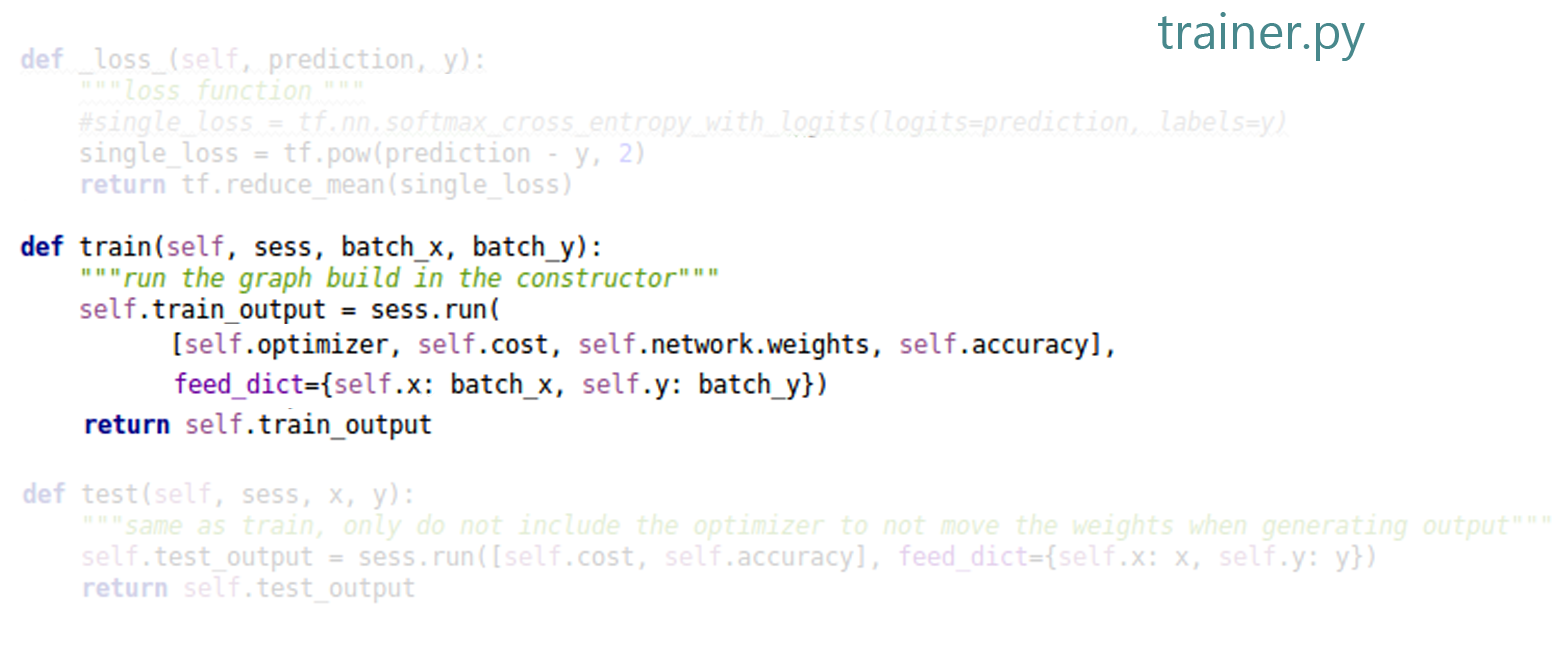
\includegraphics[width=1\textwidth]{Figures/code8_trainertrain.png}}
\end{minipage}
}
\end{frame}%}}}
 


\begin{frame}{training results - convergence}
%{{{
\linespread{1}\large{
\begin{minipage}{1\textwidth}
\begin{center}
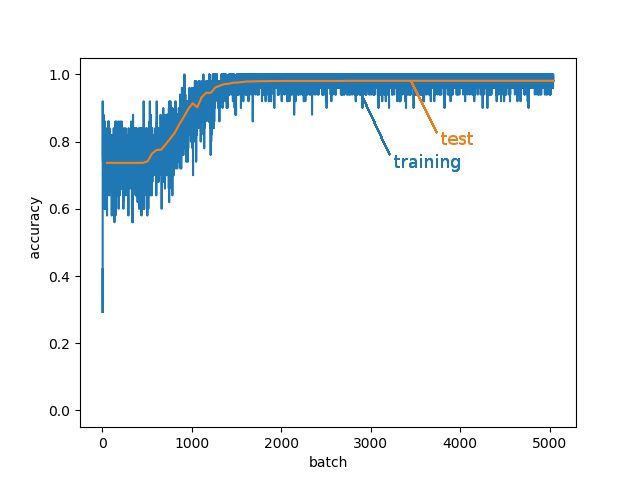
\includegraphics[width=0.8\textwidth]{Figures/StandardParseBODYKEY1.png}
\end{center}
\end{minipage}
}
\end{frame}%}}}
 
 


\begin{frame}{training results - character importance}
%{{{
\linespread{1}\large{
\begin{minipage}{1\textwidth}
\begin{center}
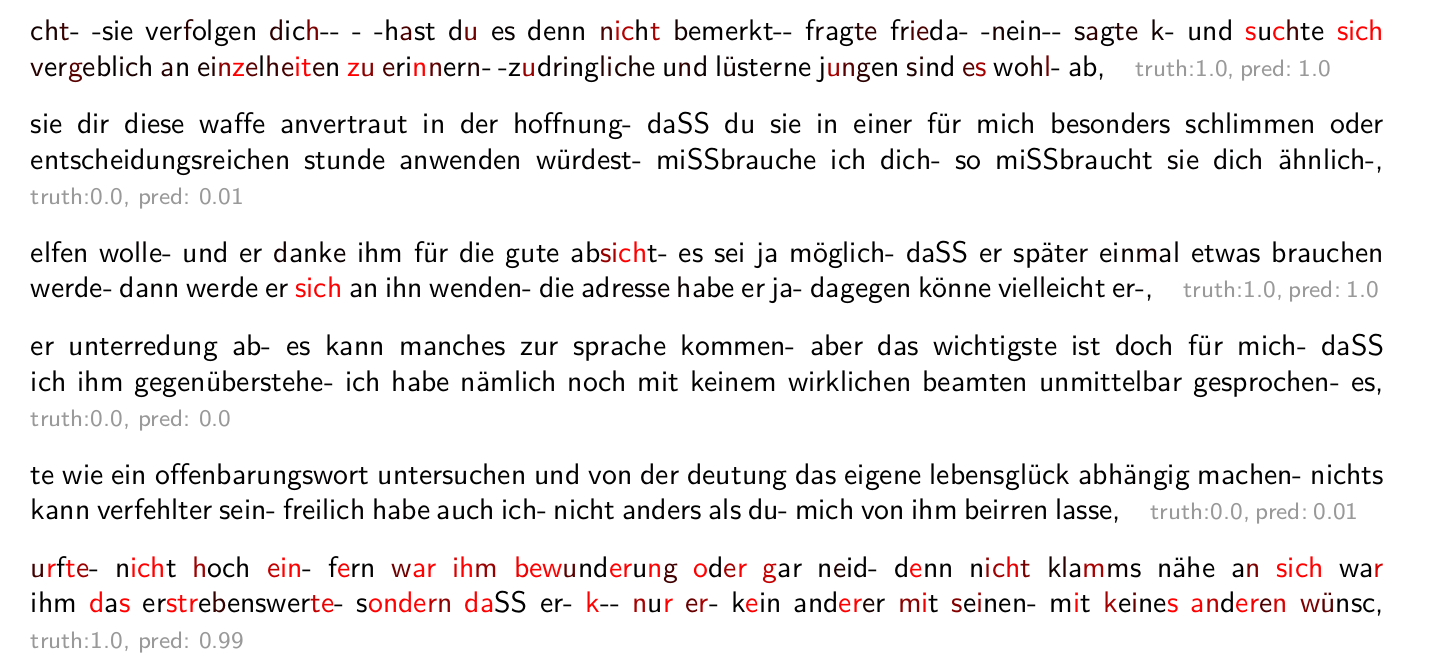
\includegraphics[width=0.99\textwidth]{Figures/ExampleText.png}
\end{center}
\end{minipage}
}
\end{frame}%}}}














 

  
 

\end{document}


















































